% =====================================================================
%  Major Project Report: Mock Interview AI
%  Compile with pdfLaTeX (Overleaf default). Run twice for the contents.
% =====================================================================
\documentclass[12pt,a4paper,oneside]{report}

% ---------------------------------------------------------------------
%  EDIT THIS BLOCK: your details appear everywhere automatically
% ---------------------------------------------------------------------
\newcommand{\projecttitle}{Mock Interview AI: An AI-Powered Mock Interview Platform with CV Analysis, Voice Interaction and Behavioural Feedback}
\newcommand{\shorttitle}{Mock Interview AI}
\newcommand{\studentnames}{STUDENT NAME 1 \quad (Roll No.: XXXXXXXX)\\ STUDENT NAME 2 \quad (Roll No.: XXXXXXXX)\\ STUDENT NAME 3 \quad (Roll No.: XXXXXXXX)}
\newcommand{\studentnamesinline}{STUDENT NAME 1 (XXXXXXXX), STUDENT NAME 2 (XXXXXXXX) and STUDENT NAME 3 (XXXXXXXX)}
\newcommand{\degreename}{Bachelor of Technology}
\newcommand{\branch}{Computer Science and Engineering}
\newcommand{\department}{Department of Computer Science and Engineering}
\newcommand{\college}{COLLEGE NAME}
\newcommand{\university}{UNIVERSITY NAME}
\newcommand{\city}{CITY}
\newcommand{\guide}{GUIDE NAME}
\newcommand{\guidedesignation}{Assistant Professor, \department}
\newcommand{\hod}{HOD NAME}
\newcommand{\session}{Session 2025--2026}
\newcommand{\submissionmonth}{MONTH YEAR}
% Optional: put your college logo at figures/logo.png and it appears on the title page.
% ---------------------------------------------------------------------

\usepackage[utf8]{inputenc}
\usepackage[T1]{fontenc}
\usepackage{amsmath}
\usepackage{newtxtext,newtxmath}
\usepackage[a4paper,left=1.25in,right=1in,top=1in,bottom=1in,headheight=15pt]{geometry}
\usepackage{setspace}
\onehalfspacing
\usepackage{graphicx}
\usepackage{float}
\usepackage{booktabs}
\usepackage{tabularx}
\usepackage{array}
\usepackage{longtable}
\usepackage{enumitem}
\usepackage[table]{xcolor}
\usepackage{listings}
\usepackage{caption}
\usepackage{fancyhdr}
\usepackage{titlesec}
\usepackage{tikz}
\usetikzlibrary{positioning,arrows.meta,shapes.geometric,shapes.misc,fit,calc,backgrounds}
\usepackage[hidelinks]{hyperref}
\usepackage{algorithm}
\usepackage{algpseudocode}

% ---------- colours (the app's palette, darkened for print) ----------
\definecolor{coral}{RGB}{220,78,78}
\definecolor{brandmagenta}{RGB}{176,52,164}
\definecolor{brandamber}{RGB}{214,138,24}
\definecolor{brandcyan}{RGB}{16,150,178}
\definecolor{ink}{RGB}{34,26,60}
\definecolor{codebg}{RGB}{247,246,251}

% ---------- headings, headers, captions ----------
\titleformat{\chapter}[display]{\normalfont\bfseries\centering}{\Large CHAPTER \thechapter}{8pt}{\LARGE}
\titlespacing*{\chapter}{0pt}{-10pt}{24pt}
\titleformat{\section}{\normalfont\large\bfseries}{\thesection}{0.8em}{}
\titleformat{\subsection}{\normalfont\normalsize\bfseries}{\thesubsection}{0.8em}{}
\pagestyle{fancy}
\fancyhf{}
\fancyhead[L]{\small\textit{\shorttitle}}
\fancyhead[R]{\small\textit{\nouppercase{\leftmark}}}
\fancyfoot[C]{\thepage}
\renewcommand{\headrulewidth}{0.4pt}
\captionsetup{font=small,labelfont=bf}
\renewcommand{\bibname}{References}
\setlist{itemsep=2pt,topsep=4pt}
\renewcommand{\arraystretch}{1.25}
\newcolumntype{Y}{>{\raggedright\arraybackslash}X}

% ---------- code listings ----------
\lstdefinelanguage{JavaScript}{
  keywords={const,let,var,function,return,if,else,for,of,in,new,async,await,try,catch,throw,break,continue,while,true,false,null,export,import,from,default},
  sensitive=true,
  comment=[l]{//},
  morecomment=[s]{/*}{*/},
  morestring=[b]',
  morestring=[b]"
}
\lstset{
  language=JavaScript,
  basicstyle=\ttfamily\footnotesize,
  keywordstyle=\color{brandmagenta}\bfseries,
  commentstyle=\color{gray}\itshape,
  stringstyle=\color{coral!80!black},
  backgroundcolor=\color{codebg},
  frame=single,
  rulecolor=\color{gray!40},
  breaklines=true,
  numbers=left,
  numberstyle=\tiny\color{gray},
  xleftmargin=2em,
  framexleftmargin=1.5em,
  showstringspaces=false,
  tabsize=2,
  columns=fullflexible,
  keepspaces=true,
  captionpos=b
}

% ---------- diagram styles ----------
\tikzset{
  box/.style={draw=ink!70, rounded corners=3pt, fill=#1, align=center, minimum height=1cm, text width=3.1cm, font=\small},
  box/.default={white},
  wide/.style={draw=ink!70, rounded corners=4pt, fill=#1, align=center, minimum height=1.2cm, text width=14cm, font=\small},
  wide/.default={white},
  ext/.style={draw=ink!60, dashed, rounded corners=3pt, fill=gray!6, align=center, minimum height=0.9cm, text width=3.1cm, font=\small},
  step/.style={draw=ink!70, rounded corners=4pt, fill=#1, align=center, minimum height=0.95cm, text width=7.5cm, font=\small},
  step/.default={coral!10},
  decision/.style={draw=ink!70, diamond, aspect=2.4, fill=brandamber!15, align=center, font=\small, inner sep=1pt},
  state/.style={draw=ink!70, circle, fill=#1, align=center, minimum size=2cm, font=\small\bfseries},
  state/.default={coral!10},
  arrow/.style={-{Stealth[length=2.5mm]}, thick, draw=ink!70},
  biarrow/.style={{Stealth[length=2.5mm]}-{Stealth[length=2.5mm]}, thick, draw=ink!70},
  lbl/.style={font=\scriptsize, fill=white, inner sep=1.5pt, align=center}
}
\newcommand{\actor}[3]{%
  \draw[thick] (#1,#2+0.55) circle (0.18);
  \draw[thick] (#1,#2+0.37) -- (#1,#2-0.15);
  \draw[thick] (#1-0.3,#2+0.2) -- (#1+0.3,#2+0.2);
  \draw[thick] (#1,#2-0.15) -- (#1-0.25,#2-0.55);
  \draw[thick] (#1,#2-0.15) -- (#1+0.25,#2-0.55);
  \node[font=\small\bfseries, align=center] at (#1,#2-0.9) {#3};}

\begin{document}

% =====================================================================
%  TITLE PAGE
% =====================================================================
\begin{titlepage}
  \centering
  {\Large\bfseries \projecttitle\par}
  \vspace{1.2cm}
  {\large A Major Project Report\par}
  \vspace{0.3cm}
  submitted in partial fulfilment of the requirements\\ for the award of the degree of\par
  \vspace{0.4cm}
  {\large\bfseries \degreename\par}
  \vspace{0.2cm}
  in\par
  \vspace{0.2cm}
  {\large\bfseries \branch\par}
  \vspace{1cm}
  Submitted by\par
  \vspace{0.3cm}
  {\bfseries \studentnames\par}
  \vspace{1cm}
  Under the guidance of\par
  \vspace{0.2cm}
  {\large\bfseries \guide\par}
  \guidedesignation\par
  \vfill
  \IfFileExists{figures/logo.png}{\includegraphics[width=3cm]{figures/logo.png}\par\vspace{0.5cm}}{}
  {\large\bfseries \department\par}
  {\large\bfseries \college\par}
  \university, \city\par
  \vspace{0.2cm}
  \session\par
\end{titlepage}

\pagenumbering{roman}
\setcounter{page}{2}

% =====================================================================
%  CERTIFICATE
% =====================================================================
\chapter*{Certificate}
\addcontentsline{toc}{chapter}{Certificate}
\thispagestyle{plain}

This is to certify that the major project report entitled \textbf{``\projecttitle''} submitted by \textbf{\studentnamesinline} to the \department, \college, \university, in partial fulfilment of the requirements for the award of the degree of \textbf{\degreename} in \textbf{\branch}, is a bonafide record of the work carried out by them under my supervision during the \session.

The matter embodied in this report has not been submitted, in part or in full, to any other university or institution for the award of any degree or diploma.

\vspace{3cm}
\noindent
\begin{tabularx}{\textwidth}{@{}X X@{}}
\rule{5cm}{0.4pt} & \hfill\rule{5cm}{0.4pt} \\
\textbf{\guide} & \hfill\textbf{\hod} \\
Project Guide & \hfill Head of Department \\
\department & \hfill \department \\
\end{tabularx}

\vspace{2cm}
\noindent Date: \rule{3.5cm}{0.4pt} \hfill Place: \city

% =====================================================================
%  DECLARATION
% =====================================================================
\chapter*{Declaration}
\addcontentsline{toc}{chapter}{Declaration}
\thispagestyle{plain}

We hereby declare that the work presented in this major project report entitled \textbf{``\projecttitle''} is an authentic record of our own work carried out under the guidance of \textbf{\guide}, \guidedesignation, \college.

The matter embodied in this report has not been submitted by us for the award of any other degree or diploma. Wherever we have used material (text, data, figures or software) from other sources, due credit has been given by citing them in the text and in the list of references.

\vspace{3cm}
\noindent\begin{tabular}{@{}l@{}}
\studentnames
\end{tabular}

\vspace{1.5cm}
\noindent Date: \rule{3.5cm}{0.4pt} \hfill Place: \city

% =====================================================================
%  ACKNOWLEDGEMENT
% =====================================================================
\chapter*{Acknowledgement}
\addcontentsline{toc}{chapter}{Acknowledgement}
\thispagestyle{plain}

We express our sincere gratitude to our project guide, \textbf{\guide}, for the continuous guidance, encouragement and valuable feedback throughout this project. Their suggestions shaped both the technical direction and the evaluation of the system.

We are thankful to \textbf{\hod}, Head of the \department, for providing the facilities and support needed to complete this work, and to all faculty members of the department for their help at various stages.

We also thank our friends and classmates who volunteered to try the mock interviews and gave honest feedback on the questions, the interface and the report. Finally, we are grateful to our families for their constant support and motivation.

\vspace{2cm}
\noindent\begin{tabular}{@{}l@{}}
\studentnames
\end{tabular}

% =====================================================================
%  ABSTRACT
% =====================================================================
\chapter*{Abstract}
\addcontentsline{toc}{chapter}{Abstract}
\thispagestyle{plain}

Job interviews decide careers, yet most candidates practise them without realistic feedback. Existing practice options are either generic question lists, peer mock interviews that depend on another person's availability, or commercial tools that ignore the candidate's own CV. This project presents \textbf{Mock Interview AI}, a browser-based platform that conducts a realistic, spoken, two-round mock interview personalised to the candidate's CV and academic record, and then produces a detailed performance report.

The candidate enters their academic record (10th, 12th or Diploma, UG, PG and PhD, each with stream and score) and uploads a CV in PDF, DOCX or text form. A large language model (Google Gemini) analyses the CV, scores it on ATS-friendliness, clarity, impact, formatting and relevance, and flags issues an interviewer is likely to probe, such as a drop in academic scores. The candidate then chooses a difficulty level (Beginner for freshers, Intermediate for 2--3 years of experience, Hard for 8+ years) and a duration: at most 90 minutes for the technical round and at most 15 minutes for a separate HR round. About two thirds of the questions are generated from specific items in the CV, and software candidates also receive coding problems drawn from a curated bank of 50 problems widely reported from FAANG interviews, solved in a built-in code editor.

The laptop speaks each question using speech synthesis, and the candidate's spoken answer is transcribed live using the browser's speech recognition. Throughout the interview, the webcam feed is analysed entirely on the device using MediaPipe Face Landmarker (478 facial landmarks and 52 expression coefficients at about 10 frames per second) to estimate eye contact, face presence, additional people in frame, smiling, facial tension, blink rate and head movement, which are combined into a confidence score. Each answer is evaluated as it is given, natural follow-up questions are asked when an answer is vague, and a final report gives an overall score, a hire verdict, per-question feedback with model answers, communication and body-language analysis, a CV review and a personalised study plan, downloadable as a PDF.

To make the system dependable on the free tier of the Gemini API, which limits each model to about 20 requests per day and frequently returns ``high demand'' errors, a resilient client was designed that automatically falls back across all available flash models, skips retired or exhausted models, enforces per-request timeouts and an overall time budget, and offers a complete rule-based Offline mode. End-to-end tests with a real API key confirmed that all five AI stages (CV analysis, technical question planning, answer evaluation, HR question planning and final report) produce correct, well-structured output. The application runs on Windows and macOS in Chrome or Edge, and has been deployed as a public HTTPS website.

\vspace{0.5cm}
\noindent\textbf{Keywords:} mock interview, large language models, Gemini, CV analysis, speech recognition, text-to-speech, facial landmarks, MediaPipe, behavioural analysis, React.

% =====================================================================
%  CONTENTS
% =====================================================================
\tableofcontents
\listoffigures
\listoftables

\chapter*{List of Abbreviations}
\addcontentsline{toc}{chapter}{List of Abbreviations}
\thispagestyle{plain}
\begin{tabularx}{\textwidth}{@{}lY@{}}
\toprule
\textbf{Abbreviation} & \textbf{Full form} \\
\midrule
AI & Artificial Intelligence \\
API & Application Programming Interface \\
ATS & Applicant Tracking System \\
CDN & Content Delivery Network \\
CGPA & Cumulative Grade Point Average \\
CV & Curriculum Vitae (resume) \\
DFD & Data Flow Diagram \\
DSA & Data Structures and Algorithms \\
FAANG & Facebook (Meta), Amazon, Apple, Netflix, Google \\
HR & Human Resources \\
HTTPS & Hypertext Transfer Protocol Secure \\
JSON & JavaScript Object Notation \\
LLM & Large Language Model \\
PDF & Portable Document Format \\
STAR & Situation, Task, Action, Result \\
STT & Speech-to-Text \\
TTS & Text-to-Speech \\
UI / UX & User Interface / User Experience \\
WASM & WebAssembly \\
WPM & Words Per Minute \\
\bottomrule
\end{tabularx}

\clearpage
\pagenumbering{arabic}

% =====================================================================
\chapter{Introduction}
% =====================================================================

\section{Background}
The interview remains the single most important step in hiring. For engineering graduates it usually has two parts: a technical or domain round that tests fundamentals, projects and, in software roles, coding ability; and an HR or behavioural round that tests communication, motivation and cultural fit. Large technology companies such as Google, Amazon and Meta have made the technical round particularly demanding, with algorithmic problems solved live while the candidate explains their reasoning aloud.

Candidates prepare mainly by reading question lists and solving problems silently on coding websites. Neither activity reproduces the real situation, in which a person asks questions out loud, listens to spoken answers, follows up on weak points, watches body language, and questions the candidate about every line of their CV. Human mock interviews are the closest substitute, but they require an experienced interviewer, are hard to schedule and rarely produce structured feedback.

Recent progress in large language models (LLMs) \cite{vaswani2017,brown2020,gemini2023}, browser speech technology \cite{webspeech} and real-time facial landmark detection \cite{lugaresi2019,kartynnik2019} makes it possible to automate a large part of this experience on an ordinary laptop.

\section{Motivation}
The project was motivated by four observations from our own placement preparation:
\begin{enumerate}
  \item Interviewers ask first about what is on the CV (projects, internships, listed skills), but generic practice tools do not read the CV at all.
  \item Speaking an answer is very different from knowing it. Candidates who can solve a problem on paper often struggle to explain it aloud under time pressure.
  \item Non-verbal behaviour (eye contact, looking down at notes, nervousness) influences interviewers, yet candidates never see measurements of their own behaviour.
  \item Freshers, mid-level engineers and senior professionals face very different interviews, so one fixed question set does not fit everyone.
\end{enumerate}

\section{Problem Statement}
To design and implement a cross-platform application that conducts a realistic, voice-based mock interview personalised to a candidate's CV, academic record and experience level, consisting of a technical round of at most 90 minutes and a separate HR round of at most 15 minutes, which analyses the candidate's answers, code and on-camera behaviour, and produces a detailed, actionable performance report together with a review of the CV.

\section{Objectives}
\begin{enumerate}
  \item Collect the candidate's academic record (10th, 12th or Diploma, UG, PG, PhD with stream and score) and CV, and analyse the CV for quality, ATS-friendliness, strengths, weaknesses and red flags.
  \item Offer three difficulty levels (Beginner, Intermediate, Hard) chosen before the interview starts.
  \item Generate interview questions of which roughly two thirds are grounded in specific CV items, and include real coding problems reported from FAANG interviews for software candidates.
  \item Speak each question aloud, capture the spoken answer as text, and support a code editor for coding questions.
  \item Analyse the webcam feed on the device for eye contact, presence, additional faces and expressions, without uploading video.
  \item Enforce hard time limits: at most 90 minutes for the technical round and at most 15 minutes for the HR round.
  \item Conduct a separate HR round after the technical round.
  \item Produce a final report with scores, per-question feedback, model answers, behavioural analysis, a CV review and a study plan, downloadable as a PDF.
  \item Run on both Windows and macOS, and remain usable when the AI service is busy or unavailable.
\end{enumerate}

\section{Scope}
The system targets students and professionals preparing for campus placements and lateral hiring in any field. Software and data roles receive coding questions; other engineering, business and science roles receive domain and case-study questions instead. The application runs entirely in a modern browser (Chrome or Edge) on Windows or macOS; no server of our own is required, because AI calls go directly from the browser to the Gemini API. The behavioural analysis is intended as practice feedback, not as a hiring decision tool.

\section{Organisation of the Report}
Chapter~\ref{ch:lit} reviews related research and existing tools. Chapter~\ref{ch:req} specifies the requirements. Chapter~\ref{ch:design} presents the architecture and design. Chapter~\ref{ch:impl} describes the implementation, including the algorithms for question planning, behavioural analysis, scoring and resilient AI access. Chapter~\ref{ch:test} reports testing, and Chapter~\ref{ch:results} presents results and discussion. Chapter~\ref{ch:conc} concludes and outlines future work.

% =====================================================================
\chapter{Literature Survey}\label{ch:lit}
% =====================================================================

\section{Structured Interviews}
Research in personnel psychology consistently finds that structured interviews, in which questions are planned in advance, tied to job requirements and scored against defined criteria, are more reliable and valid than unstructured conversations \cite{campion1997,levashina2014}. Behavioural questions answered in the STAR format (Situation, Task, Action, Result) are a common structured technique and are widely used by large employers. Our system follows these findings: every question is planned in advance with a set of expected key points, and answers are scored against those points.

\section{Automated Interview Coaching and Analysis}
Hoque et al.\ developed MACH (My Automated Conversation coacH) \cite{hoque2013}, a virtual agent that conducted mock job interviews and gave feedback on speech and facial expressions; users who practised with it showed improved interview performance as judged by human experts. Naim et al.\ \cite{naim2018} recorded mock interviews and showed that automatically extracted verbal, prosodic and facial features can predict human ratings of interview performance, with features such as speaking rate, fewer filler words and more smiling associated with better ratings. These studies established that automated behavioural feedback is feasible and useful. However, they relied on laboratory setups or offline processing and did not generate content-specific questions from the candidate's own CV.

\section{Facial Landmarks, Gaze and Blink Detection}
MediaPipe \cite{lugaresi2019} is a framework for building real-time perception pipelines that run on mobile and web platforms. Its face mesh model \cite{kartynnik2019} estimates a dense 3D surface of the face (468 points, extended to 478 with iris landmarks) from a single camera image in real time. The newer Face Landmarker task also outputs 52 blendshape coefficients describing expressions such as smiling, eye blinks and gaze direction, which correspond loosely to the action units of the Facial Action Coding System \cite{ekman1978}. Soukupov\'{a} and \v{C}ech \cite{soukupova2016} showed that simple geometric measures over eye landmarks detect blinks reliably in real time. We build on these results, using landmark geometry for head orientation and blendshape scores for gaze, blinks and expressions.

\section{Large Language Models as Interviewers and Judges}
Transformer-based language models \cite{vaswani2017} trained at scale show strong few-shot ability \cite{brown2020}, and multimodal models such as Gemini \cite{gemini2023} can read documents, including PDFs and images, directly. Zheng et al.\ \cite{zheng2023} studied LLMs as judges of open-ended answers and found that strong models agree with human preferences at a level comparable to agreement between humans, while noting biases such as a preference for longer answers. This supports using an LLM to evaluate interview answers against explicit key points, while keeping a transparent rubric.

\section{Existing Platforms}
Table~\ref{tab:existing} compares representative categories of existing practice tools with the proposed system.

\begin{table}[H]
\centering
\caption{Comparison of existing interview-practice approaches with the proposed system}
\label{tab:existing}
\small
\begin{tabularx}{\textwidth}{@{}Ycccccc@{}}
\toprule
\textbf{Approach} & \textbf{Uses CV} & \textbf{Voice} & \textbf{Camera} & \textbf{Coding} & \textbf{HR round} & \textbf{Detailed report} \\
\midrule
Question lists and books \cite{mcdowell2015} & No & No & No & Partly & Partly & No \\
Coding practice websites & No & No & No & Yes & No & Partly \\
Peer mock-interview platforms & Partly & Yes & Yes & Yes & Partly & Partly \\
Generic AI question practice tools & No & Partly & No & No & Partly & Partly \\
Research prototypes \cite{hoque2013,naim2018} & No & Yes & Yes & No & Yes & Partly \\
\textbf{Proposed system} & \textbf{Yes} & \textbf{Yes} & \textbf{Yes} & \textbf{Yes} & \textbf{Yes} & \textbf{Yes} \\
\bottomrule
\end{tabularx}
\end{table}

\section{Research Gap}
No single tool we examined combines (i) CV-driven question generation, (ii) spoken questions and answers, (iii) real coding problems in an editor, (iv) on-device behavioural analysis, (v) separate technical and HR rounds with enforced time limits, and (vi) a combined performance and CV report, while also running for free on an ordinary laptop. This project addresses that gap.

% =====================================================================
\chapter{Requirement Analysis and Specification}\label{ch:req}
% =====================================================================

\section{Functional Requirements}
\begin{table}[H]
\centering
\caption{Functional requirements}
\label{tab:fr}
\small
\begin{tabularx}{\textwidth}{@{}lY@{}}
\toprule
\textbf{ID} & \textbf{Requirement} \\
\midrule
FR1 & Accept name, optional target role and company, and the academic record: 10th, 12th or Diploma, UG, PG and PhD, each with stream and score in \%, CGPA out of 10 or CGPA out of 4. \\
FR2 & Accept a CV as PDF, DOCX, TXT or image (images in AI mode). \\
FR3 & Analyse the CV and show scores (overall, ATS, clarity, impact, formatting, relevance), skills, projects, experience, strengths, weaknesses, red flags, improvements, keywords to add and likely topics. \\
FR4 & Let the candidate choose Beginner, Intermediate or Hard, and durations of up to 90 minutes (technical) and 15 minutes (HR). \\
FR5 & Generate a technical round in which about 65\% of the questions reference specific CV items, including FAANG coding problems for software roles. \\
FR6 & Speak each question aloud and transcribe the spoken answer live; allow typing and editing as a fallback. \\
FR7 & Provide a code editor with language selection for coding questions. \\
FR8 & Analyse the webcam locally for eye contact, face presence, multiple faces, smile, tension, blinks and head movement. \\
FR9 & Evaluate each answer and ask follow-up questions when appropriate; enforce the time limits strictly. \\
FR10 & Run a separate HR round after the technical round, with the option to skip it. \\
FR11 & Generate a final report and export it as a PDF. \\
FR12 & Work without an API key (Offline mode) and fall back to Offline mode when the AI service is unavailable. \\
\bottomrule
\end{tabularx}
\end{table}

\section{Non-Functional Requirements}
\begin{itemize}
  \item \textbf{Portability:} runs on Windows and macOS in Chrome or Edge without installation beyond Node.js for local use, or with no installation at all from the hosted site.
  \item \textbf{Privacy:} video is never uploaded or stored; no interview history is kept; the API key stays in the user's browser and is excluded from the public build.
  \item \textbf{Responsiveness:} the interviewer should never stall; per-answer evaluation is limited to about 30 seconds, after which local scoring is used.
  \item \textbf{Reliability:} tolerate AI service overload, retired models and daily quota limits.
  \item \textbf{Usability:} clear step indicator, readable dark theme, keyboard shortcut (Ctrl/Cmd + Enter) to submit, and reduced motion for users who request it.
  \item \textbf{Cost:} usable on the free tier of the Gemini API, and fully usable with no key at all.
\end{itemize}

\section{Hardware and Software Requirements}
\begin{table}[H]
\centering
\caption{Hardware and software requirements}
\label{tab:hwsw}
\small
\begin{tabularx}{\textwidth}{@{}lY@{}}
\toprule
\textbf{Item} & \textbf{Requirement} \\
\midrule
Processor & Any dual-core x86-64 or Apple Silicon processor \\
Memory & 4 GB RAM minimum, 8 GB recommended \\
Peripherals & Webcam, microphone and speakers (headphones recommended) \\
Operating system & Windows 10/11 or macOS 12 and later \\
Browser & Google Chrome or Microsoft Edge (speech recognition support) \\
Runtime (local use) & Node.js 18 or later \\
Network & Internet connection for speech recognition, AI calls and first-time model download \\
AI service (optional) & Google Gemini API key (free tier supported) \\
\bottomrule
\end{tabularx}
\end{table}

\section{Feasibility Study}
\textbf{Technical feasibility.} All required capabilities are available in the browser: the Web Speech API provides text-to-speech and speech recognition \cite{webspeech}; MediaPipe runs face analysis through WebAssembly at interactive frame rates \cite{lugaresi2019}; and the Gemini REST API accepts CVs directly as PDF input \cite{gemini2023}.

\textbf{Economic feasibility.} All libraries are open source. The Gemini API has a free tier, and the application also works without it. Hosting a static site is free on common platforms. The project therefore has no mandatory running cost.

\textbf{Operational feasibility.} The candidate only needs a browser. The workflow mirrors a real interview and requires no training beyond reading the on-screen instructions.

\section{Use Case Diagram}
Figure~\ref{fig:usecase} shows the main use cases. The candidate is the primary actor; the Gemini API is a secondary actor used for analysis, question generation and evaluation.

\begin{figure}[H]
\centering
\resizebox{\linewidth}{!}{%
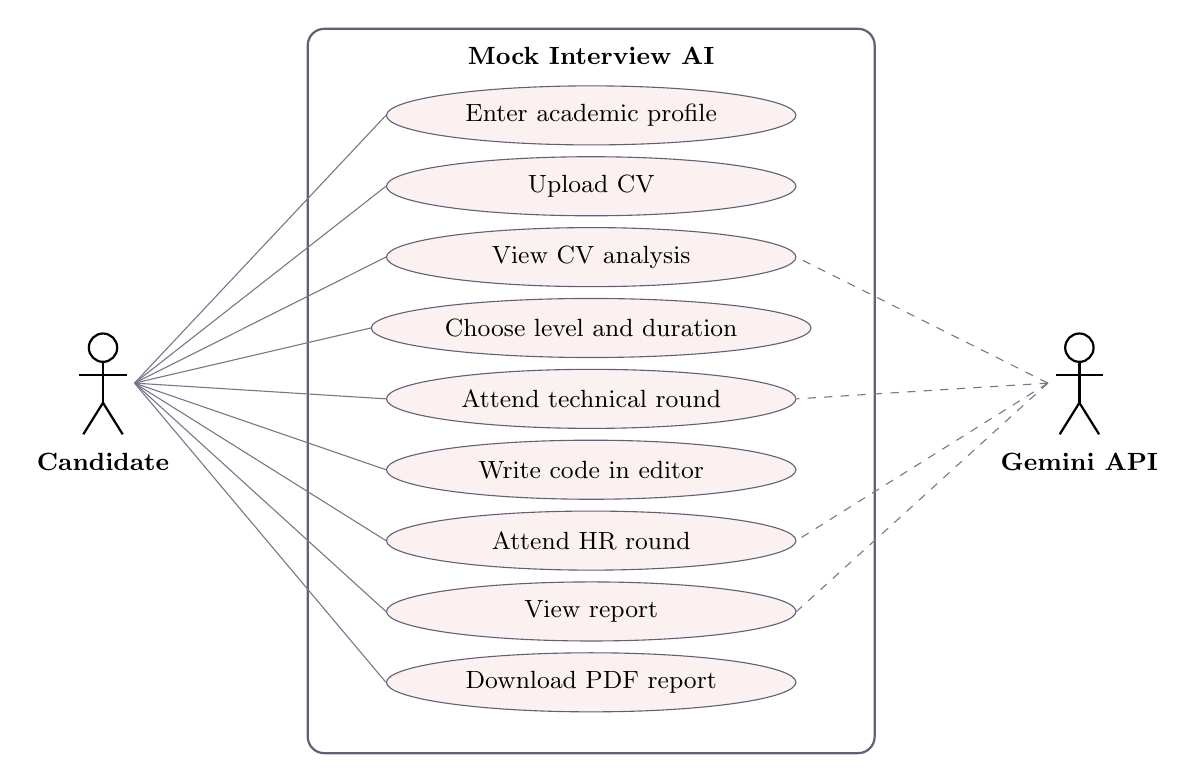
\begin{tikzpicture}
  \actor{-6.2}{0}{Candidate}
  \draw[ink!70, rounded corners=6pt, thick] (-3.6,-4.6) rectangle (3.6,4.6);
  \node[font=\small\bfseries] at (0,4.25) {Mock Interview AI};
  \tikzset{uc/.style={ellipse, draw=ink!70, fill=coral!8, minimum width=5.2cm, minimum height=0.75cm, font=\small}}
  \node[uc] (u1) at (0,3.5) {Enter academic profile};
  \node[uc] (u2) at (0,2.6) {Upload CV};
  \node[uc] (u3) at (0,1.7) {View CV analysis};
  \node[uc] (u4) at (0,0.8) {Choose level and duration};
  \node[uc] (u5) at (0,-0.1) {Attend technical round};
  \node[uc] (u6) at (0,-1.0) {Write code in editor};
  \node[uc] (u7) at (0,-1.9) {Attend HR round};
  \node[uc] (u8) at (0,-2.8) {View report};
  \node[uc] (u9) at (0,-3.7) {Download PDF report};
  \foreach \uc in {u1,u2,u3,u4,u5,u6,u7,u8,u9} \draw[ink!60] (-5.8,0.1) -- (\uc.west);
  \actor{6.2}{0}{Gemini API}
  \foreach \uc in {u3,u5,u7,u8} \draw[ink!60, dashed] (5.8,0.1) -- (\uc.east);
\end{tikzpicture}}
\caption{Use case diagram}
\label{fig:usecase}
\end{figure}

% =====================================================================
\chapter{System Design}\label{ch:design}
% =====================================================================

\section{System Architecture}
The application is a single-page web application with no custom back-end server. Figure~\ref{fig:arch} shows its layered architecture. The presentation layer consists of React components for each step. The orchestration layer holds the application state machine and the interview loop, and exposes a single facade (\texttt{interviewAI.js}) for all AI work. Below it, four services provide AI access (Gemini client and Offline engine), speech, and vision.

\begin{figure}[H]
\centering
\resizebox{\linewidth}{!}{%
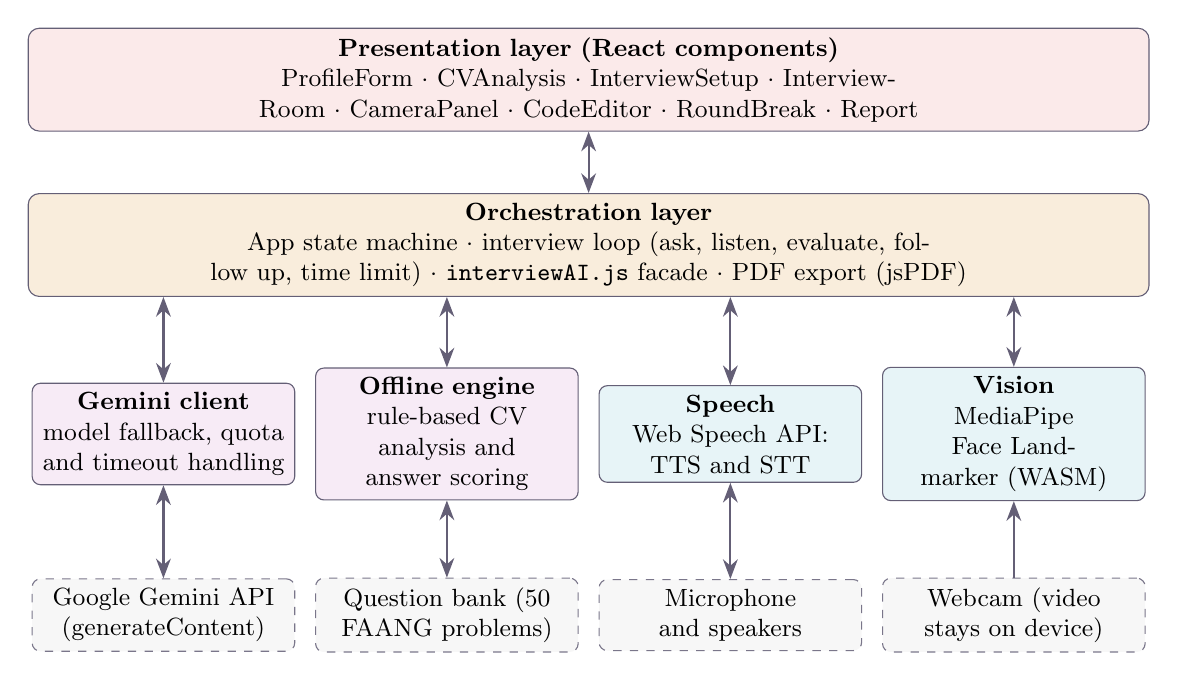
\begin{tikzpicture}
  \node[wide={coral!12}] (ui) at (0,0) {\textbf{Presentation layer (React components)}\\ ProfileForm $\cdot$ CVAnalysis $\cdot$ InterviewSetup $\cdot$ InterviewRoom $\cdot$ CameraPanel $\cdot$ CodeEditor $\cdot$ RoundBreak $\cdot$ Report};
  \node[wide={brandamber!15}] (orch) at (0,-2.1) {\textbf{Orchestration layer}\\ App state machine $\cdot$ interview loop (ask, listen, evaluate, follow up, time limit) $\cdot$ \texttt{interviewAI.js} facade $\cdot$ PDF export (jsPDF)};
  \node[box={brandmagenta!10}] (gem) at (-5.4,-4.5) {\textbf{Gemini client}\\ model fallback, quota and timeout handling};
  \node[box={brandmagenta!10}] (off) at (-1.8,-4.5) {\textbf{Offline engine}\\ rule-based CV analysis and answer scoring};
  \node[box={brandcyan!10}] (sp) at (1.8,-4.5) {\textbf{Speech}\\ Web Speech API: TTS and STT};
  \node[box={brandcyan!10}] (vis) at (5.4,-4.5) {\textbf{Vision}\\ MediaPipe Face Landmarker (WASM)};
  \node[ext] (api) at (-5.4,-6.8) {Google Gemini API (generateContent)};
  \node[ext] (bank) at (-1.8,-6.8) {Question bank (50 FAANG problems)};
  \node[ext] (dev) at (1.8,-6.8) {Microphone and speakers};
  \node[ext] (cam) at (5.4,-6.8) {Webcam (video stays on device)};
  \draw[biarrow] (ui) -- (orch);
  \foreach \n in {gem,off,sp,vis} \draw[biarrow] (orch.south -| \n.north) -- (\n.north);
  \draw[biarrow] (gem) -- (api);
  \draw[biarrow] (off) -- (bank);
  \draw[biarrow] (sp) -- (dev);
  \draw[arrow] (cam) -- (vis);
\end{tikzpicture}}
\caption{Layered system architecture}
\label{fig:arch}
\end{figure}

\section{Workflow}
Figure~\ref{fig:workflow} shows the end-to-end workflow. The order of steps is fixed, matching a real interview process.

\begin{figure}[H]
\centering
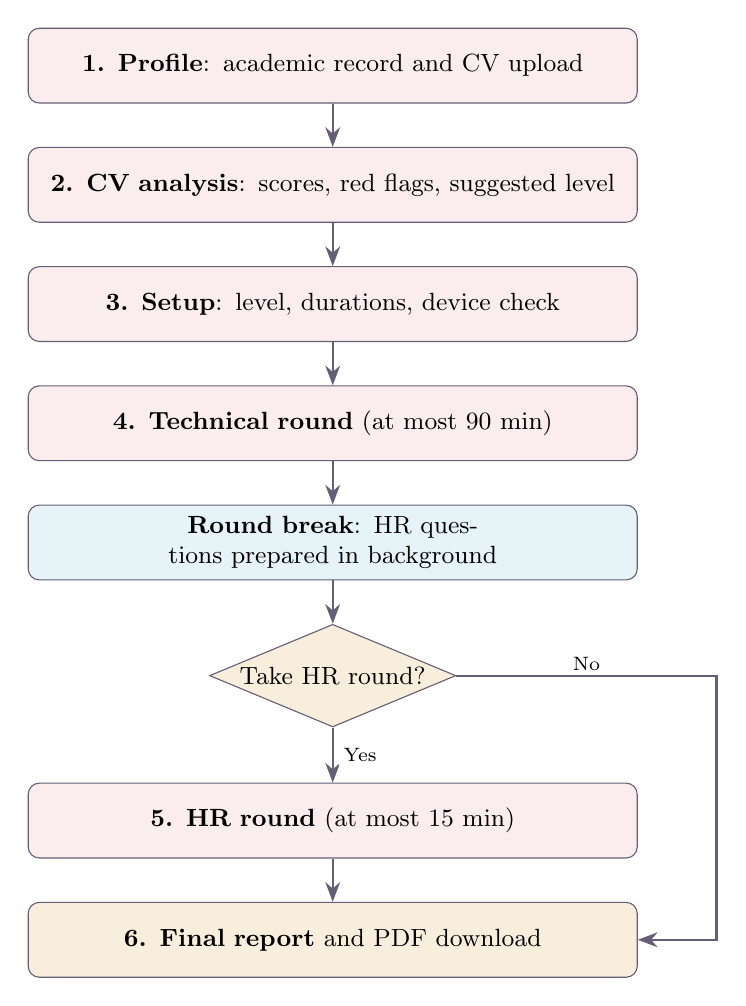
\begin{tikzpicture}[node distance=0.55cm]
  \node[step] (s1) {\textbf{1. Profile}: academic record and CV upload};
  \node[step, below=of s1] (s2) {\textbf{2. CV analysis}: scores, red flags, suggested level};
  \node[step, below=of s2] (s3) {\textbf{3. Setup}: level, durations, device check};
  \node[step, below=of s3] (s4) {\textbf{4. Technical round} (at most 90 min)};
  \node[step, below=of s4, fill=brandcyan!10] (s5) {\textbf{Round break}: HR questions prepared in background};
  \node[decision, below=of s5] (d1) {Take HR round?};
  \node[step, below=0.7cm of d1] (s6) {\textbf{5. HR round} (at most 15 min)};
  \node[step, below=of s6, fill=brandamber!15] (s7) {\textbf{6. Final report} and PDF download};
  \draw[arrow] (s1) -- (s2);
  \draw[arrow] (s2) -- (s3);
  \draw[arrow] (s3) -- (s4);
  \draw[arrow] (s4) -- (s5);
  \draw[arrow] (s5) -- (d1);
  \draw[arrow] (d1) -- node[lbl, right=2pt] {Yes} (s6);
  \draw[arrow] (s6) -- (s7);
  \draw[arrow] (d1.east) -- ($(d1.east -| s7.east)+(1,0)$) node[lbl, above, pos=0.5] {No} |- (s7.east);
\end{tikzpicture}
\caption{End-to-end workflow}
\label{fig:workflow}
\end{figure}

\section{Data Flow Diagrams}
Figure~\ref{fig:dfd0} is the context-level (level 0) data flow diagram and Figure~\ref{fig:dfd1} decomposes the system into its main processes (level 1).

\begin{figure}[H]
\centering
\resizebox{\linewidth}{!}{%
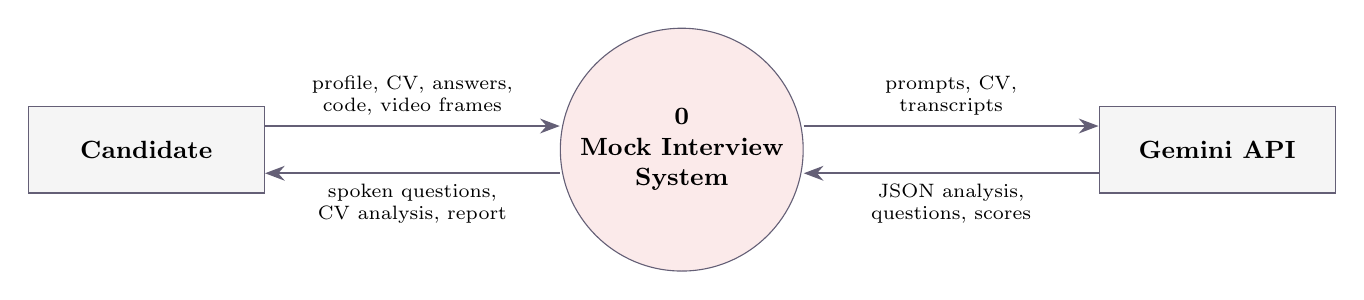
\begin{tikzpicture}
  \node[draw=ink!70, fill=gray!8, minimum width=3cm, minimum height=1.1cm, font=\small\bfseries] (cand) at (-6.8,0) {Candidate};
  \node[draw=ink!70, circle, fill=coral!12, minimum size=3cm, align=center, font=\small\bfseries] (sys) at (0,0) {0\\ Mock Interview\\ System};
  \node[draw=ink!70, fill=gray!8, minimum width=3cm, minimum height=1.1cm, font=\small\bfseries] (gem) at (6.8,0) {Gemini API};
  \draw[arrow] ([yshift=0.3cm]cand.east) -- node[lbl, above=2pt] {profile, CV, answers,\\ code, video frames} ([yshift=0.3cm]sys.west);
  \draw[arrow] ([yshift=-0.3cm]sys.west) -- node[lbl, below=2pt] {spoken questions,\\ CV analysis, report} ([yshift=-0.3cm]cand.east);
  \draw[arrow] ([yshift=0.3cm]sys.east) -- node[lbl, above=2pt] {prompts, CV,\\ transcripts} ([yshift=0.3cm]gem.west);
  \draw[arrow] ([yshift=-0.3cm]gem.west) -- node[lbl, below=2pt] {JSON analysis,\\ questions, scores} ([yshift=-0.3cm]sys.east);
\end{tikzpicture}}
\caption{Level 0 (context) data flow diagram}
\label{fig:dfd0}
\end{figure}

\begin{figure}[H]
\centering
\resizebox{\linewidth}{!}{%
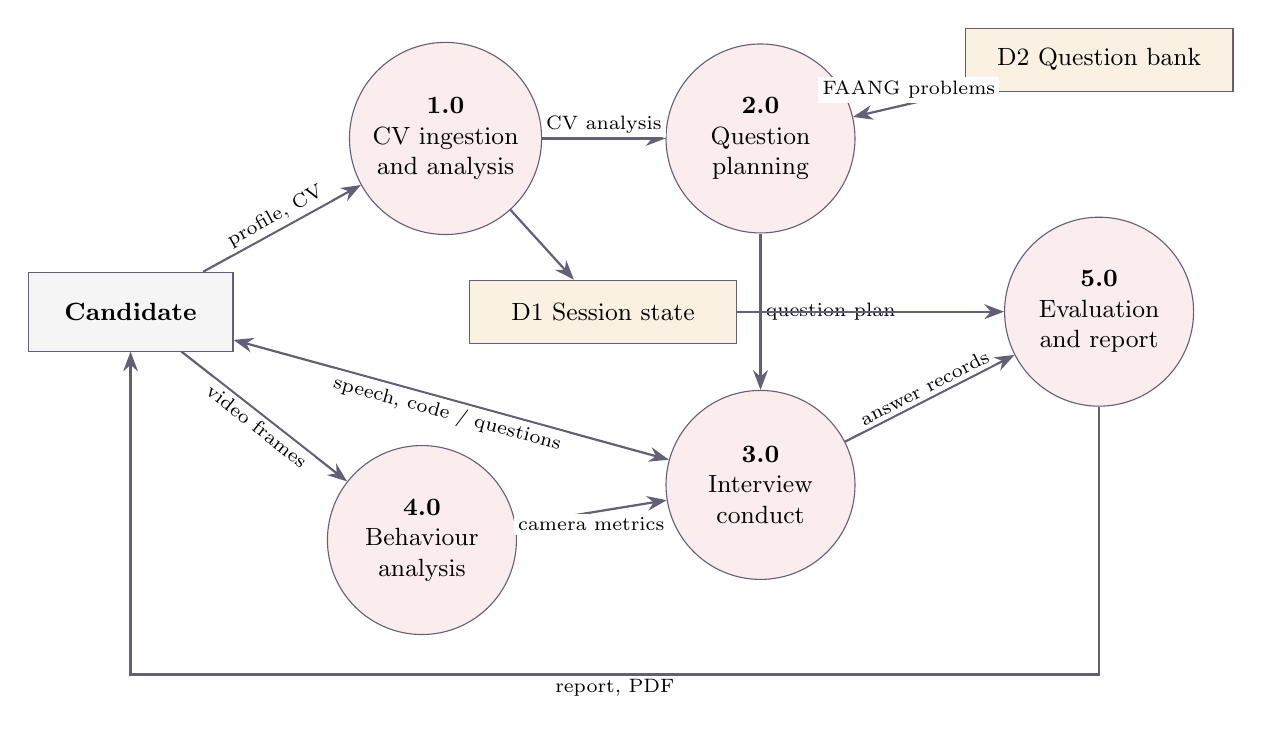
\begin{tikzpicture}
  \tikzset{proc/.style={draw=ink!70, circle, fill=coral!10, minimum size=2.4cm, align=center, font=\small}}
  \tikzset{store/.style={draw=ink!70, fill=brandamber!12, minimum width=3.4cm, minimum height=0.8cm, font=\small, align=center}}
  \node[draw=ink!70, fill=gray!8, minimum width=2.6cm, minimum height=1cm, font=\small\bfseries] (cand) at (-7.5,0) {Candidate};
  \node[proc] (p1) at (-3.5,2.2) {\textbf{1.0}\\ CV ingestion\\ and analysis};
  \node[proc] (p2) at (0.5,2.2) {\textbf{2.0}\\ Question\\ planning};
  \node[proc] (p3) at (0.5,-2.2) {\textbf{3.0}\\ Interview\\ conduct};
  \node[proc] (p4) at (-3.8,-2.9) {\textbf{4.0}\\ Behaviour\\ analysis};
  \node[proc] (p5) at (4.8,0) {\textbf{5.0}\\ Evaluation\\ and report};
  \node[store] (d1) at (-1.5,0) {D1 Session state};
  \node[store] (d2) at (4.8,3.2) {D2 Question bank};
  \draw[arrow] (cand) -- node[lbl, sloped, above] {profile, CV} (p1);
  \draw[arrow] (p1) -- node[lbl, above] {CV analysis} (p2);
  \draw[arrow] (d2) -- node[lbl, above] {FAANG problems} (p2);
  \draw[arrow] (p2) -- node[lbl, right] {question plan} (p3);
  \draw[biarrow] (cand) -- node[lbl, sloped, below] {speech, code / questions} (p3);
  \draw[arrow] (cand) -- node[lbl, sloped, below] {video frames} (p4);
  \draw[arrow] (p4) -- node[lbl, below] {camera metrics} (p3);
  \draw[arrow] (p1) -- (d1);
  \draw[arrow] (p3) -- node[lbl, sloped, above] {answer records} (p5);
  \draw[arrow] (d1) -- (p5);
  \draw[arrow] (p5.south) -- ++(0,-3.4) -| node[lbl, pos=0.25, below] {report, PDF} (cand.south);
\end{tikzpicture}}
\caption{Level 1 data flow diagram}
\label{fig:dfd1}
\end{figure}

\section{Module Design}
Table~\ref{tab:modules} lists the modules and their responsibilities.

\begin{table}[H]
\centering
\caption{Modules and responsibilities}
\label{tab:modules}
\small
\begin{tabularx}{\textwidth}{@{}lY@{}}
\toprule
\textbf{Module (file)} & \textbf{Responsibility} \\
\midrule
\texttt{App.jsx} & Step state machine, loading and error handling, Offline fallback, background, spotlight effect \\
\texttt{ProfileForm.jsx} & Landing section, academic record, CV upload and validation \\
\texttt{CVAnalysis.jsx} & Display of CV scores, skills, strengths, weaknesses, red flags and fixes \\
\texttt{InterviewSetup.jsx} & Level and duration choice, camera, microphone and voice checks \\
\texttt{InterviewRoom.jsx} & Interview loop: speak, listen, evaluate, follow up, timers, end of round \\
\texttt{CameraPanel.jsx} & Webcam capture and per-frame face analysis, live eye-contact indicator \\
\texttt{CodeEditor.jsx} & Monaco code editor with Python, Java, C++, JavaScript, C and Go \\
\texttt{Report.jsx} & Final report view and PDF download \\
\texttt{lib/gemini.js} & Gemini REST client with model fallback, timeouts, quota detection \\
\texttt{lib/prompts.js} & Prompt builders for CV analysis, plans, evaluation and the report \\
\texttt{lib/interviewAI.js} & Facade selecting Gemini or Offline engine; response normalisation \\
\texttt{lib/offlineAI.js} & Rule-based CV analysis, question planning, scoring and report \\
\texttt{lib/cvParser.js} & PDF (pdf.js), DOCX (mammoth) and text extraction \\
\texttt{lib/speech.js} & Text-to-speech with sentence chunking and cancellation \\
\texttt{lib/useSpeechRecognition.js} & Continuous speech recognition hook with auto-restart \\
\texttt{lib/faceAnalyzer.js} & Head pose, gaze, blink, smile, tension and movement metrics \\
\texttt{lib/speechMetrics.js} & Word count, words per minute and filler-word statistics \\
\texttt{lib/pdfReport.js} & Multi-page PDF generation \\
\texttt{data/questionBank.js} & 50 coding problems, 13 design problems, fundamentals, domain and HR banks \\
\bottomrule
\end{tabularx}
\end{table}

\section{Interview State Machine}
Each round is controlled by the state machine in Figure~\ref{fig:fsm}. The timer runs from the moment the round starts; when it expires, the current answer is saved and the round ends immediately, regardless of state.

\begin{figure}[H]
\centering
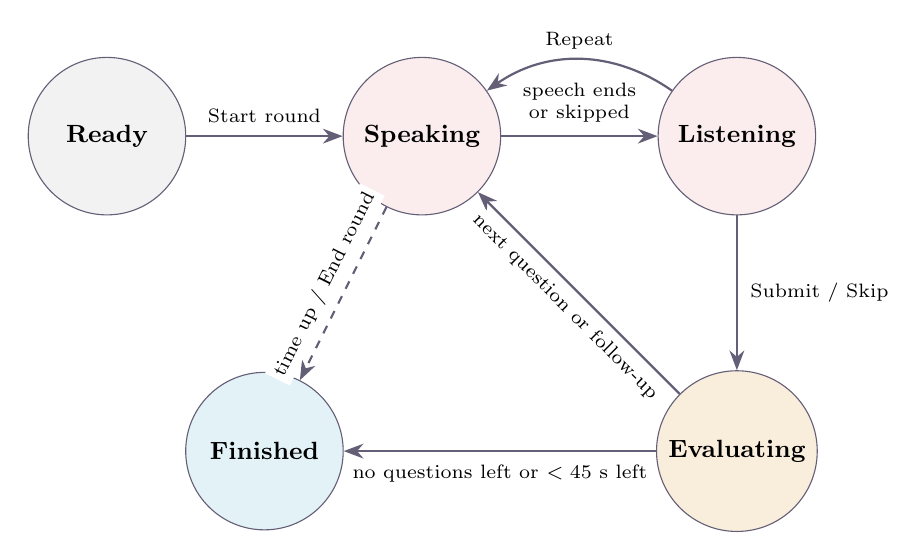
\begin{tikzpicture}
  \node[state={gray!10}] (ready) at (0,0) {Ready};
  \node[state] (speak) at (4,0) {Speaking};
  \node[state] (listen) at (8,0) {Listening};
  \node[state={brandamber!15}] (eval) at (8,-4) {Evaluating};
  \node[state={brandcyan!12}] (fin) at (2,-4) {Finished};
  \draw[arrow] (ready) -- node[lbl, above=3pt] {Start round} (speak);
  \draw[arrow] (speak) -- node[lbl, above=3pt] {speech ends\\ or skipped} (listen);
  \draw[arrow] (listen) to[bend right=35] node[lbl, above=2pt] {Repeat} (speak);
  \draw[arrow] (listen) -- node[lbl, right=3pt] {Submit / Skip} (eval);
  \draw[arrow] (eval) -- node[lbl, sloped, below=2pt] {next question or follow-up} (speak);
  \draw[arrow] (eval) -- node[lbl, below=3pt] {no questions left or $< 45$ s left} (fin);
  \draw[arrow, dashed] (speak) -- node[lbl, sloped, above=2pt] {time up / End round} (fin);
\end{tikzpicture}
\caption{Interview round state machine}
\label{fig:fsm}
\end{figure}

\section{Data Model}
The system keeps all state in memory and does not store interview history. The main records are:
\begin{itemize}
  \item \textbf{Profile:} name, target role and company, and an education object with \texttt{tenth}, \texttt{twelfth} (type 12th or Diploma), \texttt{ug}, \texttt{pg} and \texttt{phd}, each with stream, score and unit.
  \item \textbf{CV analysis:} domain, whether the role is a software role, estimated experience, suggested level, six scores, skills, experience, projects, strengths, weaknesses, red flags, improvements, missing sections, keywords to add and likely topics.
  \item \textbf{Question:} id, type (verbal or coding), category, spoken question text, full coding problem, companies known to ask it, CV reference, expected key points and suggested minutes.
  \item \textbf{Answer record:} the question fields plus transcript, code, language, duration, skip flag, per-question camera summary, speech metrics and live evaluation.
  \item \textbf{Report:} overall score, verdict, seven category scores, round summaries, per-question reviews with model answers, communication and body-language tips, CV review, academic commentary, study plan and next steps.
\end{itemize}

\section{Prompt Design}
All prompts ask the model to reply with JSON only and use Gemini's JSON response mode, so that the output can be parsed and validated reliably. Each prompt contains: a role statement (for example, a senior interviewer at a top company); the candidate block (profile, level, academic record, compact CV analysis, and the CV itself); explicit rules; and an exact output schema. Spoken questions are limited to 45 words, with no markdown or symbols, because they are read aloud by speech synthesis. The evaluation prompt tells the model to ignore minor speech-recognition errors and never reveal scores in its spoken acknowledgement. The response of every call is normalised (types coerced, scores clamped, ids reassigned), so malformed or partial responses cannot break the interface.

\section{User Interface Design}
The interface uses a deliberate dark ``stage'' theme: a deep night background with slowly drifting coloured light, a soft spotlight following the mouse pointer, and panels with gradient edges. The accent is a warm amber-to-coral-to-magenta gradient with a cyan counter-accent. Motion is used to explain state: pages fade in between steps, score rings count up, bars fill, the interviewer's avatar sends out rings while speaking, each question appears word by word, an equaliser shows while the microphone is listening, and the verdict is ``stamped'' onto the report. All animations are disabled automatically for users whose operating system requests reduced motion, and the layout collapses to a single column on phone-sized screens.

% =====================================================================
\chapter{Implementation}\label{ch:impl}
% =====================================================================

\section{Technology Stack}
\begin{table}[H]
\centering
\caption{Technology stack}
\label{tab:stack}
\small
\begin{tabularx}{\textwidth}{@{}lY@{}}
\toprule
\textbf{Technology} & \textbf{Use} \\
\midrule
React 18 & Component-based user interface \\
Vite 5 & Development server and production build \\
Google Gemini API (v1beta, \texttt{generateContent}) & CV analysis, question generation, answer evaluation, final report \\
Web Speech API & Speech synthesis (questions) and speech recognition (answers) \\
MediaPipe Tasks Vision 0.10.14 & Face Landmarker: 478 landmarks and 52 blendshapes, WebAssembly with GPU delegate \\
Monaco Editor & In-browser code editor for coding questions \\
pdf.js 4 and mammoth & Text extraction from PDF and DOCX CVs \\
jsPDF & Client-side generation of the PDF report \\
Netlify & Static HTTPS hosting of the public build \\
\bottomrule
\end{tabularx}
\end{table}

\section{CV Ingestion}
In AI mode, PDF and image CVs are sent to Gemini as inline binary data, which lets the model read scanned CVs and layouts directly. DOCX files are converted to text locally with mammoth, and plain text is sent as-is. For Offline mode, PDF text is also extracted locally with pdf.js; lines are rebuilt from text items by grouping items with the same vertical position and inserting a space where the horizontal gap between items exceeds one point.

The academic record is normalised to percentages for comparison, using the common conversions
\begin{equation}
p_{\text{CGPA}/10} = 9.5 \times g, \qquad p_{\text{CGPA}/4} = 25 \times g,
\end{equation}
and a drop of 10 or more percentage points between consecutive stages (for example 10th to 12th) is flagged as a red flag that the HR round asks about.

\section{Question Planning}
For a technical round of $T$ minutes, the number of coding problems $n_c$ and design problems $n_d$ are
\begin{equation}
n_c = \begin{cases}
0 & \text{if the role is not a software role}\\
1 & \text{if } T < 25\\
2 & \text{if } 25 \le T \le 60\\
3 & \text{if } T > 60
\end{cases}
\qquad
n_d = \begin{cases}
1 & \text{if software, level} \neq \text{Beginner and } T \ge 30\\
0 & \text{otherwise.}
\end{cases}
\end{equation}
Coding problems take 12--15 minutes at Beginner level and 15--20 minutes otherwise. The prompt requires the suggested times of all questions to add up to between $0.8T$ and $T$, and about 65\% of the questions to name a specific CV item. For each interview, a random pool of problems matching the level (for example 7 easy and 3 medium for Beginner) is drawn from the question bank and given to the model, which keeps the classic problem and records the companies known to ask it. The first question is always a warm-up about the candidate's most relevant project. HR rounds have 3, 5 or 7 questions for 5, 10 or 15 minutes, open with ``Tell me about yourself'', ask about the red flags found in the CV, and close with ``Do you have any questions for us?''.

\section{Interview Orchestration}
The interview loop implements the state machine of Figure~\ref{fig:fsm}. Key rules are:
\begin{itemize}
  \item A follow-up question is inserted after an answer only if the evaluator proposes one, the current question is not itself a follow-up, fewer than 4 (technical) or 2 (HR) follow-ups have been asked, and more than 4 minutes remain.
  \item A new coding problem is not started when fewer than 8 minutes remain, and the round ends when fewer than 45 seconds remain.
  \item When the timer expires or the candidate ends the round, the answer in progress is saved and later scored.
  \item Speech recognition is paused while the interviewer speaks, so the microphone does not transcribe the interviewer's own voice.
\end{itemize}

\section{Speech Processing}
Text-to-speech splits long questions into chunks of at most about 180 characters at sentence boundaries, because some browsers stop speaking long utterances after about 15 seconds. Utterance objects are kept referenced until they finish so that their completion events are not lost, and a safety timer ends speech if the browser never reports completion. Speech recognition runs in continuous mode with interim results. Because browsers stop recognition after periods of silence, the hook restarts it automatically while the candidate is still answering, and any words still in the interim buffer when recognition stops are kept.

From each transcript the system computes word count, speaking rate and filler words:
\begin{equation}
\text{WPM} = \frac{N_{\text{words}}}{t_{\text{answer}} / 60},
\end{equation}
computed only for spoken (non-coding) answers longer than 8 seconds and 5 words. Thirteen filler expressions such as ``um'', ``basically'' and ``you know'' are counted, and the rate per 100 words is reported.

\section{Behavioural Analysis with Computer Vision}
Each camera frame is processed at about 10 frames per second by MediaPipe Face Landmarker, configured to detect up to three faces and to output blendshapes. Head orientation is estimated from landmark ratios: nose tip (index 1), cheeks (234 and 454), forehead (10) and chin (152):
\begin{equation}
r_{\text{yaw}} = \frac{x_{1} - x_{234}}{x_{454} - x_{234}}, \qquad
r_{\text{pitch}} = \frac{y_{1} - y_{10}}{y_{152} - y_{10}}.
\end{equation}
Because people sit at different angles to their camera, the system calibrates to the candidate. It takes the running mean $(\bar r_{\text{yaw}}, \bar r_{\text{pitch}})$ over the first 20 frames in which the candidate appears to face the screen. The head is considered turned away when
\begin{equation}
\lvert r_{\text{yaw}} - \bar r_{\text{yaw}} \rvert > 0.14 \quad \text{or} \quad \lvert r_{\text{pitch}} - \bar r_{\text{pitch}} \rvert > 0.10 .
\end{equation}
The eyes are considered to look away when the blink coefficient is below 0.45 and the averaged gaze coefficients exceed 0.55 sideways, 0.55 downwards or 0.6 upwards. A frame counts as ``looking away'' if either test holds. Smiling (mouth-smile coefficient above 0.35), tension (brow-down or mouth-press above 0.45), blinks (rising edges of the blink coefficient above 0.5), additional faces and missing faces are also counted. Head movement is the mean nose displacement between frames normalised by face width, classified as low ($<0.008$), moderate ($<0.02$) or high.

Gaze tracking is paused during coding questions, because looking down at the editor is expected. The estimated confidence score combines eye contact $E$, face presence $F$, tension $T$, movement score $M$ (100, 75 or 45 for low, moderate or high movement) and smile rate $S$, all in percent:
\begin{equation}
C = 0.40\,E + 0.20\,F + 0.15\,(100 - T) + 0.10\,M + 0.15\,\min(100,\; 4S).
\end{equation}
Metrics are accumulated for each question and for each round. No video frame leaves the device.

Listing~\ref{lst:frame} shows the core of the per-frame analysis.

\begin{lstlisting}[caption={Per-frame head-pose and gaze analysis (simplified from \texttt{faceAnalyzer.js})},label={lst:frame}]
export function analyzeFrame(result, calib) {
  const faces = result?.faceLandmarks?.length || 0;
  if (!faces) return { faces: 0 };
  const lm = result.faceLandmarks[0];
  const bs = blendshapeMap(result.faceBlendshapes[0]);
  const nose = lm[1], left = lm[234], right = lm[454];
  const top = lm[10], chin = lm[152];
  const yaw = (nose.x - left.x) / (right.x - left.x);
  const pitch = (nose.y - top.y) / (chin.y - top.y);
  const blink = avg(bs.eyeBlinkLeft, bs.eyeBlinkRight);
  const gazeDown = avg(bs.eyeLookDownLeft, bs.eyeLookDownRight);
  const eyesAway = blink < 0.45 && (gazeSide(bs) > 0.55 || gazeDown > 0.55);
  calibrate(calib, yaw, pitch, eyesAway);     // first 20 frontal frames
  const headAway = Math.abs(yaw - calib.yaw) > 0.14
                || Math.abs(pitch - calib.pitch) > 0.10;
  return { faces, away: headAway || eyesAway, blink: blink > 0.5,
           smile: avg(bs.mouthSmileLeft, bs.mouthSmileRight) };
}
\end{lstlisting}

\section{Resilient Access to the AI Service}
During development we found that the free tier of the Gemini API is limited to about 20 requests per model per day, that individual models frequently respond with ``high demand'' (HTTP 503) for minutes at a time, that a model can occasionally hang for two minutes before failing, and that the model originally used (\texttt{gemini-2.5-flash}) had been retired for new keys. A single-model client was therefore not usable. Algorithm~\ref{alg:fallback} shows the client that was designed instead.

\begin{algorithm}[H]
\caption{Resilient Gemini request with model fallback}
\label{alg:fallback}
\begin{algorithmic}[1]
\Require prompt $P$, preferred model $m_0$, per-request timeout $\tau$, overall budget $B$
\State $L \gets$ unique list: last working model, $m_0$, \texttt{gemini-flash-latest}, \texttt{gemini-3-flash-preview}, \texttt{gemini-flash-lite-latest}, then all other available flash models, newest first
\State $t_{\text{end}} \gets \text{now} + B$
\For{pass $= 1$ to $2$}
  \For{each model $m \in L$ that is not retired and not exhausted}
    \For{attempt $= 1$ to $2$}
      \If{$t_{\text{end}} - \text{now} < 3$ s} \State \textbf{break} \EndIf
      \State $r \gets$ \Call{Generate}{$m, P, \min(\tau,\, t_{\text{end}} - \text{now})$}
      \If{$r$ succeeded} \State remember $m$ as last working model \State \Return parsed JSON of $r$ \EndIf
      \If{status $\in \{400, 401, 403\}$} \State \textbf{raise} request or key error \EndIf
      \If{status $= 404$} \State mark $m$ retired; \textbf{break} \EndIf
      \If{status $= 429$ with a daily quota violation} \State mark $m$ exhausted; \textbf{break} \EndIf
      \If{status $\in \{429, 500, 502, 503, 504\}$} \State \textbf{break} \Comment{try next model} \EndIf
      \State wait 1.2 s \Comment{network error or malformed JSON: retry once}
    \EndFor
  \EndFor
  \State wait 3 s
\EndFor
\State \textbf{raise} ``all models busy'' or ``daily quota used up'' \Comment{UI offers Offline mode}
\end{algorithmic}
\end{algorithm}

The per-request timeout and budget depend on the task: 60 s and 75 s for CV analysis and question planning, 20 s and 30 s for per-answer evaluation (which then falls back to local scoring so the interview never stalls), and 90 s and 180 s for the final report. Quick evaluation calls request a low ``thinking'' level from models that support it, to reduce latency. When a request fails, the interface shows the reason with \textbf{Retry} and \textbf{Continue in Offline mode} buttons.

\section{Offline Engine}
The Offline engine makes the whole application usable without any API key and serves as a fallback when the AI service is unavailable.

\textbf{CV analysis.} The CV text is split into sections using a list of common headings (Education, Experience, Projects, Skills and so on). About 160 skills in nine domain groups are matched with word boundaries; the group with the most matches determines the domain, and a software or data target role forces a software classification. Experience is estimated from explicit phrases such as ``5+ years'' or from year ranges in the experience section. The six CV scores are computed from observable signals, for example
\begin{align}
\text{Impact} &= \operatorname{clamp}_{[5,100]}\bigl(20 + 10q + 3\min(a, 15) - 4w\bigr),\\
\text{Clarity} &= \operatorname{clamp}_{[30,95]}\bigl(88 - 3w - 2\min(f, 10) - 15[\,N > 1200\,] - 15[\,N < 200\,]\bigr),
\end{align}
where $q$ is the number of lines with measurable results, $a$ the number of action verbs, $w$ the number of weak phrases such as ``responsible for'', $f$ the number of first-person pronouns and $N$ the word count. The ATS score adds points for contact details, standard sections, suitable length and bullet points; the overall score is the mean of the five component scores.

\textbf{Answer scoring.} Each expected key point is split into keywords (longer than two characters, excluding stop words); a point counts as covered when at least a third of its keywords appear in the answer or code. With coverage $c$, length factor $\ell = \min(1, N/90)$ and structure factor $s$ (1 if the answer uses connectives such as ``because'' or ``for example'', otherwise 0.4), a spoken answer scores
\begin{equation}
\text{score}_{\text{verbal}} = 10\,(0.55\,c + 0.30\,\ell + 0.15\,s),
\end{equation}
and a coding answer with $k$ non-whitespace code characters scores
\begin{equation}
\text{score}_{\text{coding}} = 10\,\bigl(0.45\,c + 0.25\min(1, k/150) + 0.20\min(1, N/50) + 0.10\,s\bigr).
\end{equation}

\textbf{Overall score.} Category scores are combined with weights of 0.30 (technical knowledge), 0.20 (problem solving), 0.10 (coding), 0.15 (communication), 0.10 (HR), 0.05 (body language) and 0.10 (CV alignment), renormalised over the categories that apply. The verdict is \emph{Strong Hire} for 85 and above, \emph{Hire} for 72--84, \emph{Lean Hire} for 60--71, \emph{Lean No Hire} for 45--59 and \emph{No Hire} below 45. All Offline results are clearly labelled as estimates in the interface and the PDF.

\section{Report Generation}
In AI mode the complete transcript (questions, answers, code, live evaluations, per-question camera metrics and speech metrics) and the CV are sent to the model with a rubric and an output schema; the model returns the verdict, category scores, round summaries, a review and a concise model answer for every question, communication and body-language tips, a CV review including whether the answers supported the CV's claims, and a study plan. The report is rendered in the browser and exported with jsPDF as a multi-page A4 document with score bars, per-question reviews, code excerpts and page numbers. Text is normalised to the Latin-1 character set supported by the PDF's built-in fonts.

\section{Deployment}
The production build is a static set of files (about 3 MB) produced by Vite. It is deployed to Netlify as a public HTTPS site, which is required for browsers to allow camera and microphone access. The developer's API key is kept in a local \texttt{.env} file. During deployment we found that the build tool reads this file even when the variable is overridden, so the first shareable build accidentally contained the key; the process was changed to build without the file and to scan the output automatically for the key before every upload. The public build therefore starts in Offline mode, and visitors can add their own free key in Settings, where it stays in their own browser.

% =====================================================================
\chapter{Testing}\label{ch:test}
% =====================================================================

\section{Testing Strategy}
Testing combined (i) production builds after every change, (ii) end-to-end tests of the complete workflow driven in a browser in Offline mode, (iii) a verification script that ran the application's own AI modules against the real Gemini API with patient retries, (iv) degradation tests with the camera and microphone blocked, and (v) responsive-layout and deployment checks.

\section{Test Cases}
\begin{table}[H]
\centering
\caption{Executed test cases}
\label{tab:tests}
\footnotesize
\begin{tabularx}{\textwidth}{@{}lYYc@{}}
\toprule
\textbf{ID} & \textbf{Test} & \textbf{Expected result} & \textbf{Status} \\
\midrule
TC01 & Complete workflow in Offline mode: profile, CV analysis, setup, technical round, break, report & Every step reached in order, report shown & Pass \\
TC02 & Text CV with 21 skills, 2 projects, 2 roles & Skills, projects and roles detected; 92\% to 74\% dip flagged & Pass \\
TC03 & CGPA 8.1/10 entered for UG & Converted to about 77\% and shown as 8.1 CGPA/10 & Pass \\
TC04 & Camera access blocked & Clear message; interview continues & Pass \\
TC05 & Microphone access blocked & Clear message; typed answers accepted & Pass \\
TC06 & Coding question in 15-minute round & Monaco editor loads; code saved and scored & Pass \\
TC07 & ``End round'' while answering & Answer saved and scored in report & Pass (after fix D1) \\
TC08 & 15-minute technical plan & Includes warm-up, a CV question and a coding problem & Pass (after fix D2) \\
TC09 & 5-minute HR plan & 3 questions, including the academic-dip question & Pass \\
TC10 & PDF export & Multi-page PDF file generated (18.7 KB) & Pass \\
TC11 & All five AI stages with real API key & Valid, well-structured JSON output at every stage & Pass \\
TC12 & Preferred model overloaded (503) or retired (404) & Automatic fallback to another model & Pass \\
TC13 & All models busy & Error with Retry and Offline buttons within 77 s & Pass \\
TC14 & ``Continue in Offline mode'' after failure & Analysis completes offline & Pass \\
TC15 & Phone width (390 px) & Single column, no horizontal scrolling & Pass \\
TC16 & Public deployment & HTTPS page loads (HTTP 200); API key absent from files & Pass \\
TC17 & Production build & Build completes without errors & Pass \\
\bottomrule
\end{tabularx}
\end{table}

\section{Verification of the AI Pipeline}
A script loaded the application's own modules (the same prompts, client and parsing code used in the browser) and ran all five AI stages against the Gemini API with a real key, retrying each stage for up to 12 attempts with 20-second pauses. Table~\ref{tab:gemini} shows the result. All stages passed; the number of attempts reflects service overload at the time of testing, not errors in the application.

\begin{table}[H]
\centering
\caption{AI pipeline verification with a real Gemini API key}
\label{tab:gemini}
\small
\begin{tabularx}{\textwidth}{@{}lcYc@{}}
\toprule
\textbf{Stage} & \textbf{Attempts} & \textbf{Model that answered} & \textbf{Elapsed (cumulative)} \\
\midrule
CV analysis & 1 & \texttt{gemini-3.5-flash-lite} & 72 s \\
Technical question plan & 3 & \texttt{gemini-3-flash-preview} & 311 s \\
Answer evaluation & 1 & \texttt{gemini-3.6-flash} & 339 s \\
HR question plan & 9 & \texttt{gemini-3.1-flash-lite-preview} & 1111 s \\
Final report & 1 & \texttt{gemini-3.1-flash-lite-preview} & 1123 s \\
\bottomrule
\end{tabularx}
\end{table}

The quality of the output was checked manually:
\begin{itemize}
  \item The 30-minute technical plan contained 6 questions whose suggested times added up to exactly 30 minutes; 4 of the 6 referred to named CV items, including a cache-invalidation question about the Redis optimisation claimed in the CV; two were coding problems tagged with the companies known to ask them, and one was a rate-limiter design question.
  \item The evaluation of a sample answer gave 8/10, correctly noted that the answer did not justify the choice of database, and proposed a relevant follow-up question.
  \item The HR plan asked about the drop from 92\% (10th) to 74\% (12th), used Amazon's ``Ownership'' leadership principle, and ended with the candidate's questions.
  \item The final report detected that a deliberately wrong solution (a hash map for ``Product of Array Except Self'') was incorrect, scored it 2/10 and explained the correct prefix and suffix product approach with its complexity. A review was produced for every question and the review ids matched the answers.
\end{itemize}

\section{Defects Found and Fixed}
\begin{table}[H]
\centering
\caption{Defects found during testing}
\label{tab:defects}
\footnotesize
\begin{tabularx}{\textwidth}{@{}lYY@{}}
\toprule
\textbf{ID} & \textbf{Defect} & \textbf{Fix} \\
\midrule
D1 & An answer cut off by the timer or ``End round'' was scored 0 & Unscored answers are scored when the report is built \\
D2 & A 15-minute round contained no CV-based question & At least one CV question is always planned \\
D3 & Summaries showed a coding question's spoken intro & The problem title is shown instead \\
D4 & Warm-up and introduction answers ignored in CV alignment & Included in the CV-alignment score \\
D5 & Skill names displayed as ``Node.Js'', duplicate ``Spring'' & Display-name table; generic term dropped when a specific one matches \\
D6 & Default model retired for new API keys & Auto-updating alias plus fallback chain \\
D7 & Misleading ``model not found'' error when all models were busy & Retired models tracked separately; busy reason reported \\
D8 & A model could hang for 120 s & Per-request timeout and overall time budget \\
D9 & API key included in the first shareable build & Build without the key file; automatic scan before upload \\
D10 & Public site required a hosting-team login & Access protection disabled for this site only \\
D11 & Step indicator overflowed the header & Compact connectors, hidden scrollbar \\
\bottomrule
\end{tabularx}
\end{table}

\section{Tests to Be Executed on Target Hardware}
The following tests require physical devices and should be recorded by the team on their own machines before the final demonstration.

\begin{table}[H]
\centering
\caption{Tests to execute on target hardware}
\label{tab:todo}
\footnotesize
\begin{tabularx}{\textwidth}{@{}lYY@{}}
\toprule
\textbf{ID} & \textbf{Test} & \textbf{Observed result} \\
\midrule
HT1 & Upload a real PDF CV & \\
HT2 & Upload a real DOCX CV & \\
HT3 & Speech recognition of spoken answers in Chrome on Windows & \\
HT4 & Speech recognition in Edge on Windows and Chrome on macOS & \\
HT5 & Eye-contact indicator changes when looking away from the screen & \\
HT6 & ``Multiple faces'' warning when a second person enters the frame & \\
HT7 & Timer ends a 90-minute technical round automatically & \\
\bottomrule
\end{tabularx}
\end{table}

% =====================================================================
\chapter{Results and Discussion}\label{ch:results}
% =====================================================================

\section{Application Screens}
Figures~\ref{fig:landing} to \ref{fig:mobile} show the implemented application. The screenshots were taken during testing in a browser in which camera and microphone access were blocked, which is why the camera panel shows a notice.

\begin{figure}[H]
\centering
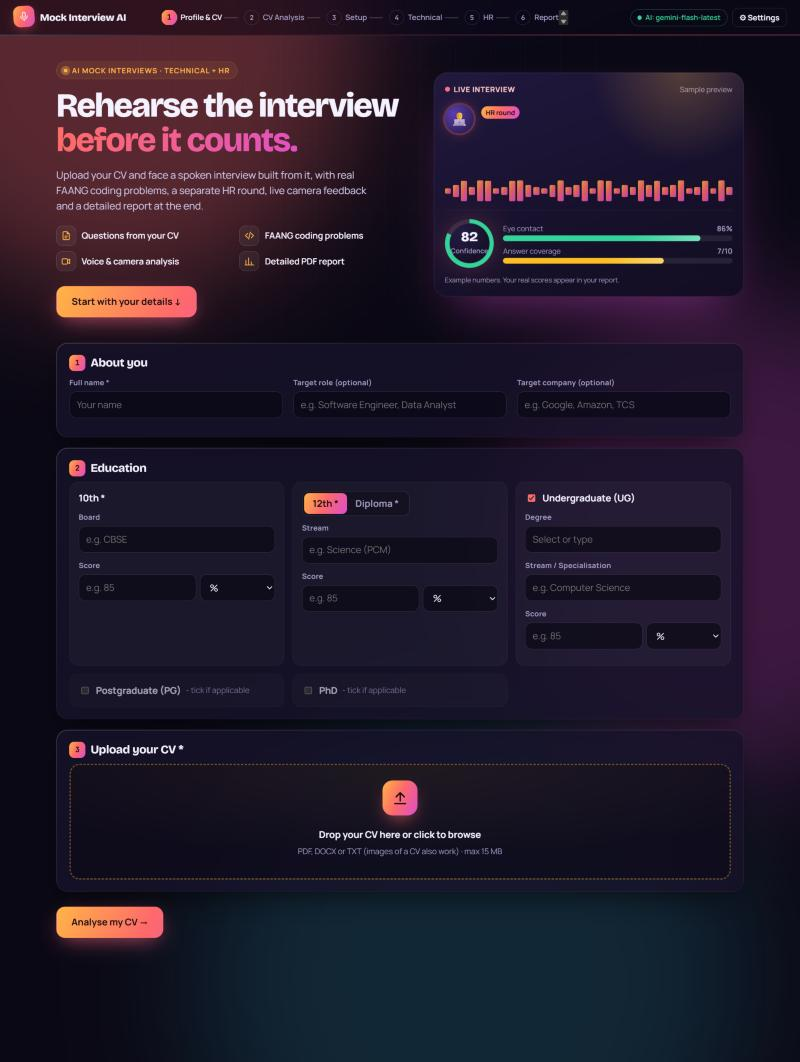
\includegraphics[width=0.85\linewidth,height=0.62\textheight,keepaspectratio]{figures/landing_page.jpg}
\caption{Landing page with the animated sample interview and the profile form}
\label{fig:landing}
\end{figure}

\begin{figure}[H]
\centering
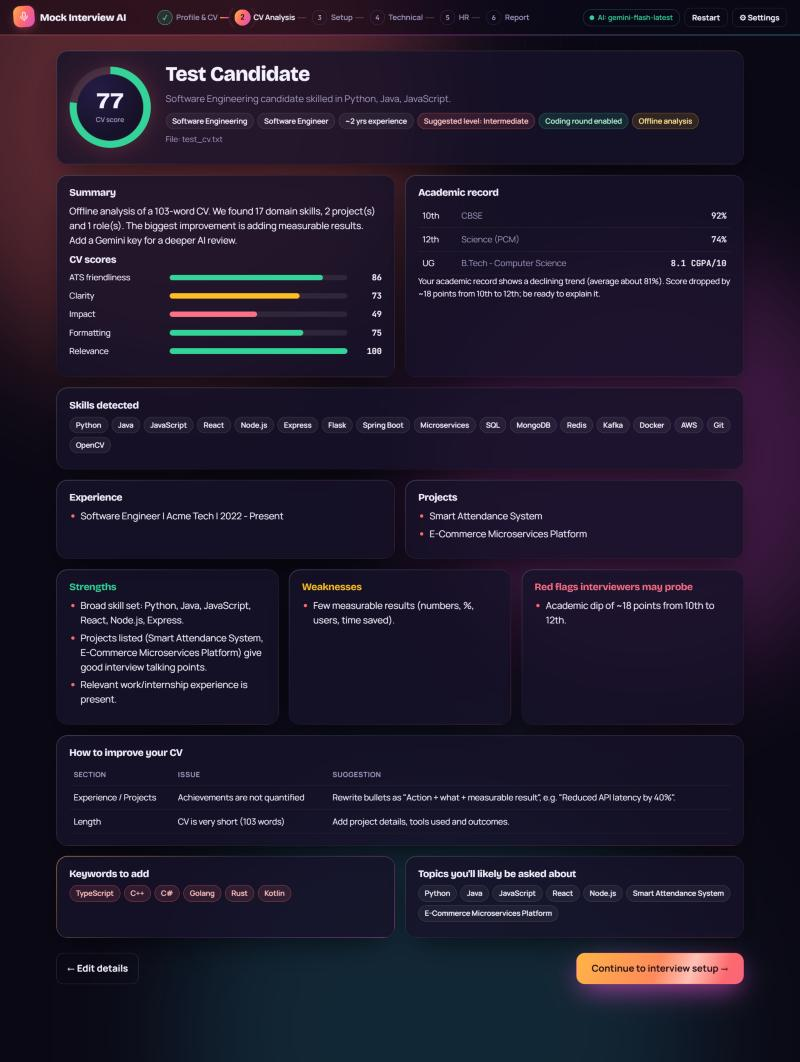
\includegraphics[width=0.85\linewidth,height=0.62\textheight,keepaspectratio]{figures/cv_analysis.jpg}
\caption{CV analysis: score ring, component scores, academic record, skills, strengths, weaknesses, red flags and suggested fixes}
\label{fig:cvanalysis}
\end{figure}

\begin{figure}[H]
\centering
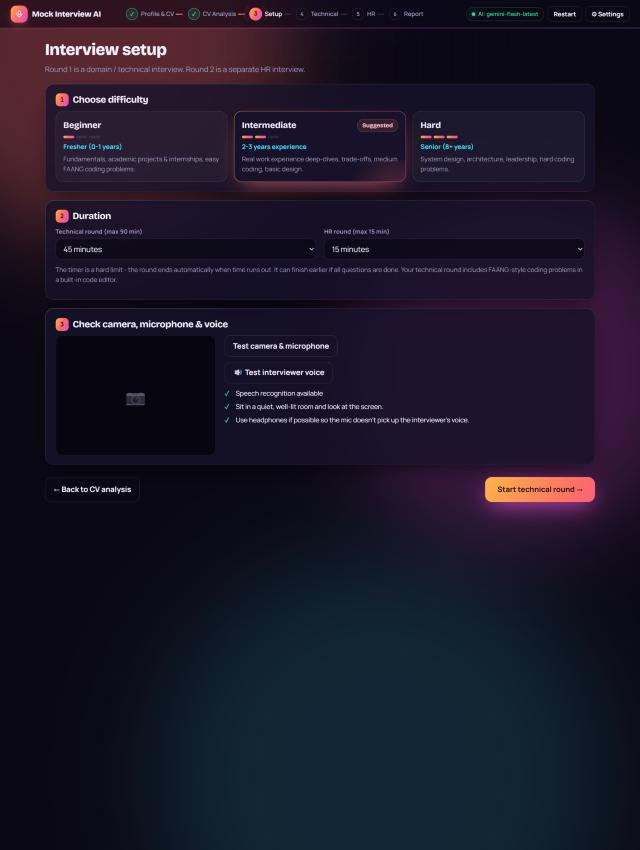
\includegraphics[width=0.85\linewidth,height=0.55\textheight,keepaspectratio]{figures/interview_setup.jpg}
\caption{Interview setup: difficulty level, round durations and device check}
\label{fig:setup}
\end{figure}

\begin{figure}[H]
\centering
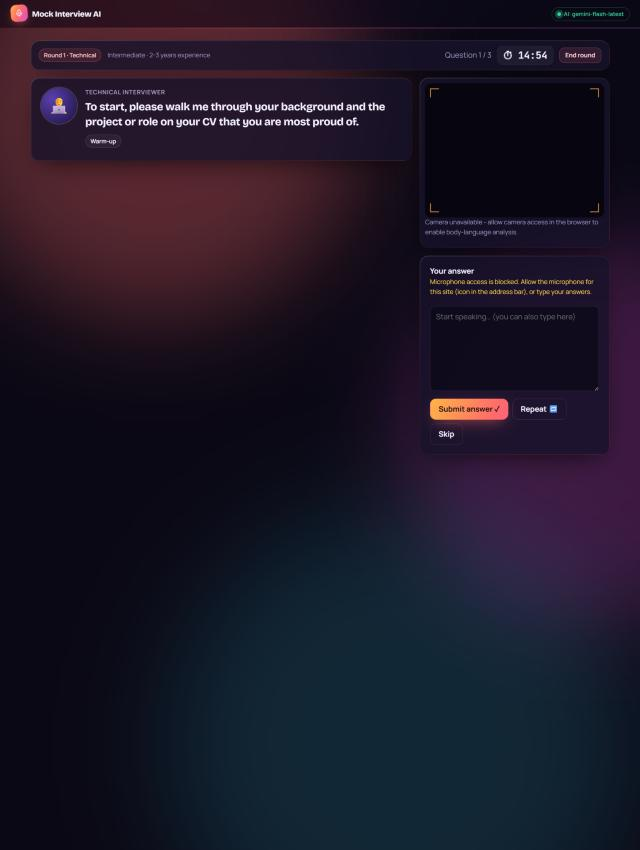
\includegraphics[width=0.85\linewidth,height=0.55\textheight,keepaspectratio]{figures/interview_room.jpg}
\caption{Interview room: spoken question, timer, camera panel and answer area}
\label{fig:room}
\end{figure}

\begin{figure}[H]
\centering
\begin{minipage}{0.48\linewidth}
  \centering
  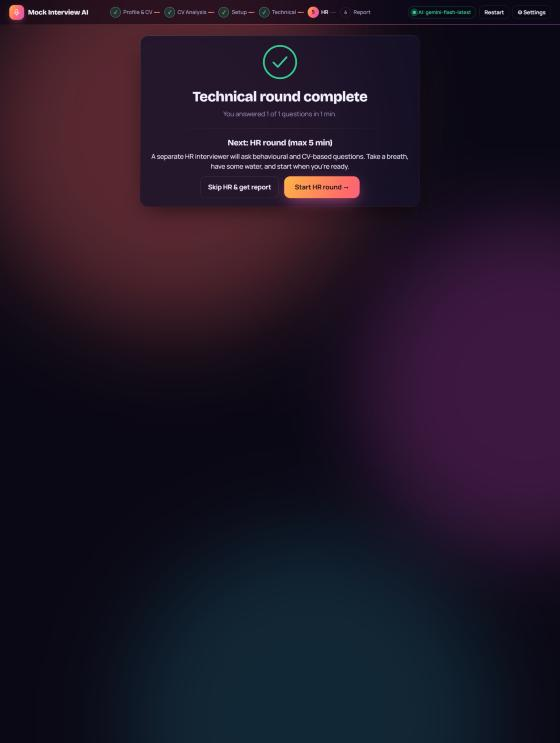
\includegraphics[width=\linewidth]{figures/round_break.jpg}
\end{minipage}\hfill
\begin{minipage}{0.48\linewidth}
  \centering
  
\includegraphics[width=\linewidth]{figures/loading_screen.jpg}
\end{minipage}
\caption{Left: break between the technical and HR rounds. Right: loading screen with interview tips while the report is generated}
\label{fig:break}
\end{figure}

\begin{figure}[H]
\centering
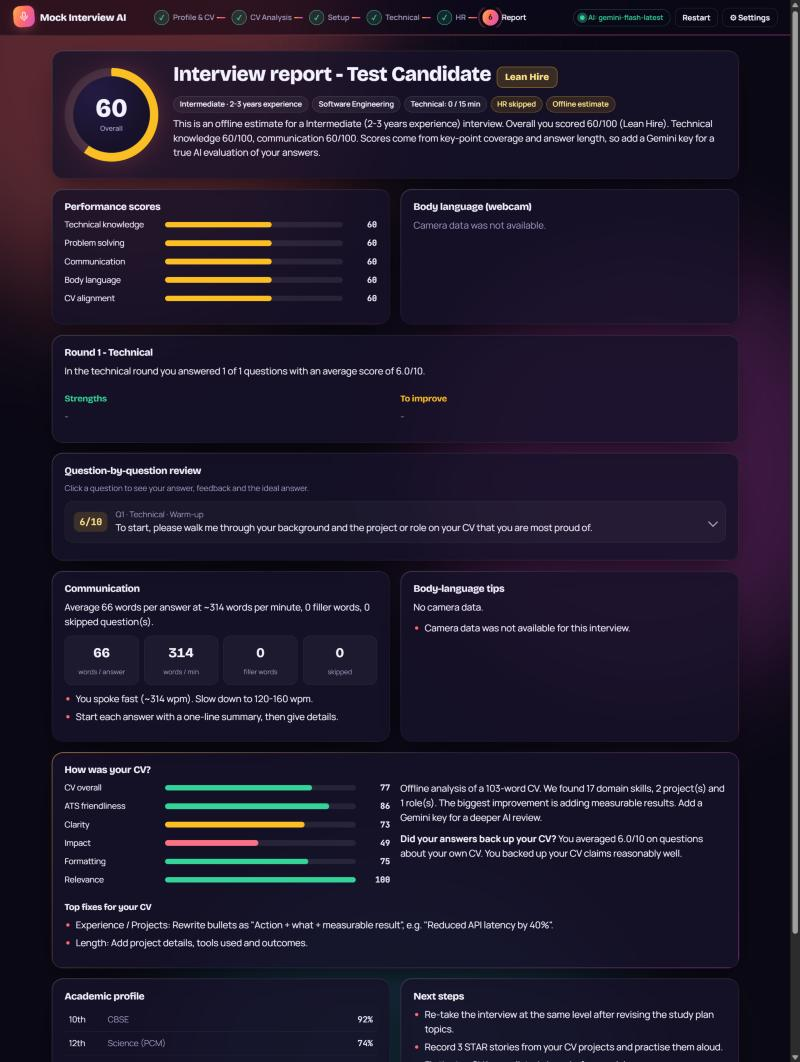
\includegraphics[width=0.85\linewidth,height=0.62\textheight,keepaspectratio]{figures/final_report.jpg}
\caption{Final report (Offline-mode estimate shown): overall score, verdict, category scores, round summary, question review, communication and CV review}
\label{fig:report}
\end{figure}

\begin{figure}[H]
\centering
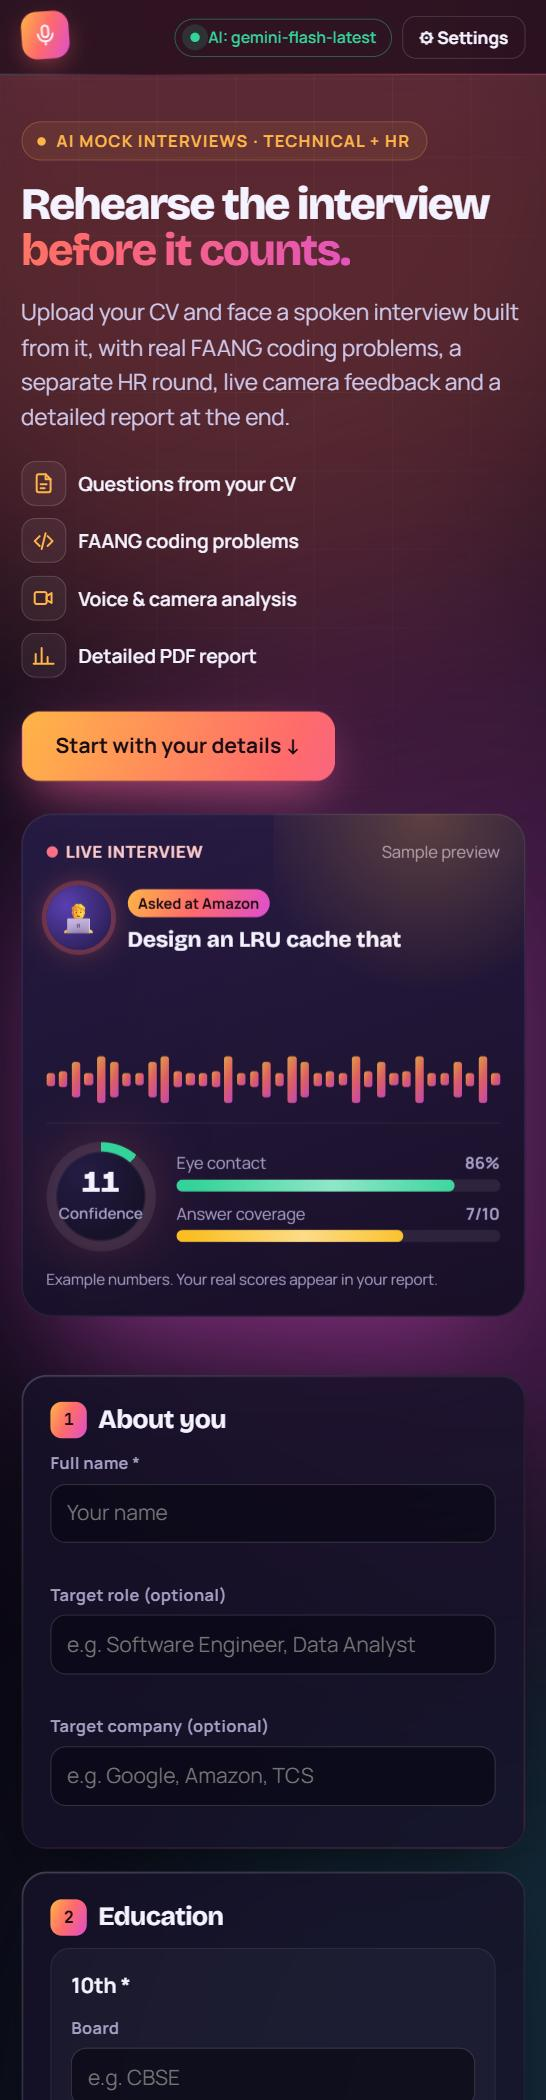
\includegraphics[height=0.6\textheight,keepaspectratio]{figures/mobile_view.jpg}
\caption{Responsive layout at phone width (390 px)}
\label{fig:mobile}
\end{figure}

\section{Sample AI Output}
The following questions were generated by the system for a test CV describing a software engineer with two years of experience, an e-commerce microservices project using Kafka, and a Redis caching optimisation (Intermediate level, 30 minutes):

\begin{enumerate}
  \item \emph{(Warm-up, CV)} ``Could you walk me through your E-Commerce Microservices Platform? Why did you choose Kafka for event streaming, and how did you ensure data consistency across your MongoDB instances?''
  \item \emph{(CV experience, asked at Amazon and Adobe)} ``At Acme Tech you reduced page load by 40 percent using Redis caching. Can you explain your cache invalidation strategy, and how you handled cache stampedes during peak traffic?''
  \item \emph{(Fundamentals, linked to CV skills)} ``Explain the difference between a process and a thread, and how it affects the design of a Node.js API compared with a multi-threaded Spring Boot application.''
  \item \emph{(FAANG coding, asked at Amazon, Meta and Apple)} Product of Array Except Self, in linear time without division.
  \item \emph{(FAANG coding)} Contains Duplicate, with a discussion of hash-set versus sorting trade-offs.
  \item \emph{(System design, asked at Google, Amazon and Stripe)} ``How would you design a rate limiter for an API at Amazon-scale traffic?''
\end{enumerate}

The questions are specific to the CV, appropriate to the level, and their suggested durations fill the chosen 30 minutes exactly.

\section{Discussion}
\textbf{Personalisation.} The main difference from generic practice tools is that most questions are about the candidate's own work. In our tests the model consistently turned CV claims (for example ``reduced page load by 40\%'') into probing questions, which is how experienced interviewers behave.

\textbf{Evaluation quality.} The live evaluator and the final report identified both correct reasoning and errors, including an incorrect coding approach, and produced concrete model answers. Using explicit expected key points for every question keeps the rubric transparent.

\textbf{Latency and availability.} The dominant practical limitation is the free tier of the AI service: in our tests individual stages sometimes needed several attempts, and the HR plan needed nine. The resilient client and the Offline fallback keep the interview usable, and live evaluation never blocks the interview for more than about 30 seconds.

\textbf{Behavioural metrics.} The camera metrics are heuristics based on published landmark and blendshape outputs, and are useful as relative practice feedback (for example, noticing frequent downward glances that suggest reading notes). They have not been validated against expert human ratings in this project, and they are presented as estimates.

\textbf{Privacy.} Video never leaves the device, no interview data is stored, and the public build contains no API key.

\section{Limitations}
\begin{itemize}
  \item Speech recognition relies on the browser's online service and works in Chrome and Edge, not Firefox.
  \item The free AI tier allows about 20 requests per model per day, while a full interview uses about 20 requests; heavy use needs a paid key or falls back to Offline mode.
  \item Offline scoring is keyword-based and cannot judge the correctness of reasoning or code.
  \item Code is reviewed but not executed against test cases.
  \item Behavioural metrics are uncalibrated heuristics and can be affected by lighting, camera position and glasses.
\end{itemize}

% =====================================================================
\chapter{Conclusion and Future Scope}\label{ch:conc}
% =====================================================================

\section{Conclusion}
This project delivered Mock Interview AI, a cross-platform, browser-based system that conducts a realistic two-round mock interview. It reads the candidate's CV and academic record, analyses and scores the CV, and adapts to three experience levels. Most questions are generated from the candidate's own CV, and software candidates also receive FAANG-reported coding problems in a built-in editor. Questions are spoken aloud and answers transcribed live, while on-device computer vision measures eye contact, presence and expressions without uploading video. A strict 90-minute technical round is followed by a separate 15-minute HR round, and a detailed report with model answers, behavioural analysis, a CV review and a study plan is produced and exported as a PDF.

Beyond the core features, the project solved the practical problem of building a dependable product on an overloaded, rate-limited free AI service, through automatic model fallback, quota awareness, time budgets and a complete Offline mode. All AI stages were verified with a real API key, and the system is deployed as a public website.

\section{Future Scope}
\begin{itemize}
  \item Execute submitted code against hidden test cases in a sandbox and include pass rates in the score.
  \item Validate the behavioural metrics against ratings by human interviewers and calibrate the thresholds.
  \item Add prosodic analysis (pitch, volume, pauses) from the audio signal.
  \item Store interview history (with consent) to show progress over time.
  \item Support more languages for questions and answers, including Indian languages.
  \item Add company-specific interview formats and a panel mode with several interviewer personas.
  \item Package the application as a desktop app for fully offline use with local speech recognition.
\end{itemize}

% =====================================================================
%  REFERENCES
% =====================================================================
\begin{thebibliography}{99}
\addcontentsline{toc}{chapter}{References}

\bibitem{campion1997} M.~A. Campion, D.~K. Palmer and J.~E. Campion, ``A review of structure in the selection interview,'' \emph{Personnel Psychology}, vol.~50, no.~3, pp.~655--702, 1997.

\bibitem{levashina2014} J.~Levashina, C.~J. Hartwell, F.~P. Morgeson and M.~A. Campion, ``The structured employment interview: Narrative and quantitative review of the research literature,'' \emph{Personnel Psychology}, vol.~67, no.~1, pp.~241--293, 2014.

\bibitem{hoque2013} M.~E. Hoque, M.~Courgeon, J.-C. Martin, B.~Mutlu and R.~W. Picard, ``MACH: My Automated Conversation coacH,'' in \emph{Proc. ACM International Joint Conference on Pervasive and Ubiquitous Computing (UbiComp)}, 2013, pp.~697--706.

\bibitem{naim2018} I.~Naim, M.~I. Tanveer, D.~Gildea and M.~E. Hoque, ``Automated analysis and prediction of job interview performance,'' \emph{IEEE Transactions on Affective Computing}, vol.~9, no.~2, pp.~191--204, 2018.

\bibitem{lugaresi2019} C.~Lugaresi \emph{et al.}, ``MediaPipe: A framework for building perception pipelines,'' arXiv:1906.08172, 2019.

\bibitem{kartynnik2019} Y.~Kartynnik, A.~Ablavatski, I.~Grishchenko and M.~Grundmann, ``Real-time facial surface geometry from monocular video on mobile GPUs,'' in \emph{CVPR Workshop on Computer Vision for Augmented and Virtual Reality}, 2019.

\bibitem{soukupova2016} T.~Soukupov\'{a} and J.~\v{C}ech, ``Real-time eye blink detection using facial landmarks,'' in \emph{Proc. 21st Computer Vision Winter Workshop}, 2016.

\bibitem{ekman1978} P.~Ekman and W.~V. Friesen, \emph{Facial Action Coding System}. Palo Alto, CA: Consulting Psychologists Press, 1978.

\bibitem{vaswani2017} A.~Vaswani \emph{et al.}, ``Attention is all you need,'' in \emph{Advances in Neural Information Processing Systems (NeurIPS)}, 2017.

\bibitem{brown2020} T.~B. Brown \emph{et al.}, ``Language models are few-shot learners,'' in \emph{Advances in Neural Information Processing Systems (NeurIPS)}, 2020.

\bibitem{gemini2023} Gemini Team, Google, ``Gemini: A family of highly capable multimodal models,'' arXiv:2312.11805, 2023.

\bibitem{zheng2023} L.~Zheng \emph{et al.}, ``Judging LLM-as-a-judge with MT-Bench and Chatbot Arena,'' in \emph{Advances in Neural Information Processing Systems (NeurIPS), Datasets and Benchmarks Track}, 2023.

\bibitem{webspeech} W3C Audio Community Group, ``Web Speech API,'' Draft Community Group Report. [Online]. Available: \url{https://webaudio.github.io/web-speech-api/}

\bibitem{mcdowell2015} G.~Laakmann McDowell, \emph{Cracking the Coding Interview}, 6th ed. Palo Alto, CA: CareerCup, 2015.

\bibitem{kleppmann2017} M.~Kleppmann, \emph{Designing Data-Intensive Applications}. Sebastopol, CA: O'Reilly Media, 2017.

\bibitem{geminidocs} Google, ``Gemini API documentation.'' [Online]. Available: \url{https://ai.google.dev/gemini-api/docs}

\bibitem{mediapipedocs} Google, ``MediaPipe Face Landmarker guide.'' [Online]. Available: \url{https://ai.google.dev/edge/mediapipe/solutions/vision/face_landmarker}

\bibitem{react} Meta Open Source, ``React documentation.'' [Online]. Available: \url{https://react.dev}

\end{thebibliography}

% =====================================================================
%  APPENDICES
% =====================================================================
\appendix

\chapter{User Manual}
\section{Running Locally}
\begin{enumerate}
  \item Install Node.js 18 or later from \url{https://nodejs.org}.
  \item Optionally create a file \texttt{.env} in the project folder containing \texttt{VITE\_GEMINI\_API\_KEY=your-key} (a free key is available from Google AI Studio). Without a key the application runs in Offline mode.
  \item On Windows, double-click \texttt{start-windows.bat}; on macOS, run \texttt{chmod +x start-mac.command} once and then double-click \texttt{start-mac.command}. Alternatively run \texttt{npm install} and \texttt{npm start}.
  \item Open \url{http://localhost:5173} in Chrome or Edge and allow camera and microphone access.
\end{enumerate}

\section{Taking an Interview}
\begin{enumerate}
  \item Fill in your name and academic record, upload your CV and click \textbf{Analyse my CV}.
  \item Review the CV analysis and click \textbf{Continue to interview setup}.
  \item Choose a level and the durations, test your camera, microphone and voice, and click \textbf{Start technical round}.
  \item Listen to each question and answer aloud. Your words appear in the answer box, where you can also type or edit. Click \textbf{Submit answer} or press Ctrl/Cmd + Enter.
  \item For coding questions, write your solution in the editor while explaining your approach aloud.
  \item After the technical round, start the HR round or skip it.
  \item Read your report and click \textbf{Download PDF report}.
\end{enumerate}

\chapter{FAANG Coding Question Bank}
Table~\ref{tab:bank} lists the 50 coding problems in the built-in question bank. They are classic problems widely reported from interviews at large technology companies; the problem statements in the application are paraphrased.

\begin{table}[H]
\centering
\caption{Coding problems in the question bank by difficulty}
\label{tab:bank}
\scriptsize
\begin{tabularx}{\textwidth}{@{}YYY@{}}
\toprule
\textbf{Easy (16)} & \textbf{Medium (22)} & \textbf{Hard (12)} \\
\midrule
Two Sum & Longest Substring Without Repeating Characters & Trapping Rain Water \\
Valid Parentheses & LRU Cache & Merge k Sorted Lists \\
Merge Two Sorted Lists & Number of Islands & Median of Two Sorted Arrays \\
Best Time to Buy and Sell Stock & Group Anagrams & Word Ladder \\
Valid Anagram & Top K Frequent Elements & Serialize and Deserialize Binary Tree \\
Reverse Linked List & Product of Array Except Self & Minimum Window Substring \\
Maximum Depth of Binary Tree & 3Sum & Sliding Window Maximum \\
Contains Duplicate & Merge Intervals & Alien Dictionary \\
Binary Search & Course Schedule & Find Median from Data Stream \\
Climbing Stairs & Binary Tree Level Order Traversal & Edit Distance \\
Linked List Cycle & Validate Binary Search Tree & Longest Increasing Path in a Matrix \\
Invert Binary Tree & Kth Largest Element in an Array & Word Search II \\
Missing Number & Coin Change & \\
Majority Element & Longest Palindromic Substring & \\
Move Zeroes & Search in Rotated Sorted Array & \\
First Unique Character in a String & Lowest Common Ancestor of a Binary Tree & \\
 & Rotting Oranges & \\
 & Subarray Sum Equals K & \\
 & Word Break & \\
 & Clone Graph & \\
 & Container With Most Water & \\
 & Meeting Rooms II & \\
\bottomrule
\end{tabularx}
\end{table}

The bank also contains 11 system design problems (for example a URL shortener, rate limiter, news feed, chat application and ride-hailing service), 2 low-level design problems (parking lot and elevator), 14 computer-science fundamentals questions, 28 domain questions for mechanical, electrical, electronics, civil, finance, marketing and general roles, and a bank of HR and behavioural questions. Every item includes the key points of a strong answer, which are used for offline scoring and in the report.

\chapter{Excerpt of the CV Analysis Prompt}
\begin{lstlisting}[language={},caption={Output schema requested for CV analysis (excerpt)},label={lst:prompt}]
Return JSON exactly in this shape:
{
  "candidateName": string,
  "headline": string,
  "domain": string,
  "isSoftwareRole": boolean,
  "estimatedExperienceYears": number,
  "suggestedLevel": "beginner" | "intermediate" | "hard",
  "summary": string,
  "scores": { "overall": int, "ats": int, "clarity": int,
              "impact": int, "formatting": int, "relevance": int },
  "skills": { "technical": [string], "tools": [string], "soft": [string] },
  "projects": [ { "name": string, "tech": [string], "summary": string } ],
  "academicTrend": string,
  "strengths": [string], "weaknesses": [string], "redFlags": [string],
  "improvements": [ { "section": string, "issue": string, "suggestion": string } ],
  "keywordsToAdd": [string], "likelyInterviewTopics": [string]
}
Rules: reference actual CV content, be specific. Scores are integers 0-100.
\end{lstlisting}

\end{document}
